\documentclass[11pt]{article}
\usepackage{geometry}
\geometry{a4paper}
%\geometry{landscape}
\usepackage[parfill]{parskip}    % Activate to begin paragraphs with an empty line rather than an indent
\usepackage{graphicx}
\usepackage{amssymb}
\usepackage{epstopdf}
\usepackage{fancyhdr}
\usepackage{fullpage}
\usepackage{appendix}
\usepackage{newclude}
\usepackage{datetime}
\usepackage{hyperref}
\usepackage{breakurl}
\usepackage{color}
\usepackage{multind}
\usepackage{microtype}
\usepackage{tabularx}
\usepackage[dutch]{babel}

\makeindex{pve}
\newcommand{\pve}[1]{ }
\newcommand{\pvelist}[1]{  }

\makeindex{drupalpath}
\newcommand{\drupalpath}[1]{\index{drupalpath}{#1}\url{gemeente.nl/#1}}



\hypersetup{
    colorlinks,
    citecolor=black,
    filecolor=black,
    linkcolor=black,
    urlcolor=black
}

\DeclareGraphicsRule{.tif}{png}{.png}{`convert #1 `dirname #1`/`basename #1 .tif`.png}

\newcommand{\seeone}[1]{ (zie \ref{#1} p.\pageref{#1})}
\newcommand{\seetwo}[2]{ (zie \ref{#1} p.\pageref{#1},  \ref{#2} p.\pageref{#2})}

\pagestyle{fancy}
\fancyhead{}
\fancyfoot{}
\fancyfoot[R]{\thepage}

\setcounter{secnumdepth}{5}
\setcounter{tocdepth}{5}

\makeatletter
\renewcommand\paragraph{%
   \@startsection{paragraph}{4}{0mm}%
      {-\baselineskip}%
      {.5\baselineskip}%
      {\normalfont\normalsize\bfseries}}
\makeatother

\newcommand{\customer}{Dimpact }
\newcommand{\thecustomer}{\customer }
\newcommand{\customerdomain}{dimpact.nl}
\newcommand{\customerdomainuc}{Dimpact.nl}

\title{Handleiding \customerdomainuc}
\author{Mike Hens \\ Maurits Lawende \\ Patrick Kraaij \\ Maarten Hartman \\ David van Dijk \\ Marc Kwee \\ Eric Alvares}
\date{}

\begin{document}
\maketitle
\begin{center}
%
\includegraphics{img/logo.jpg}

Laatst bijgewerkt: \\ \ddmmyyyydate \today
\end{center}
\pagebreak

\renewcommand*\contentsname{Inhoudsopgave}
\tableofcontents
\pagebreak


\section{Site inleiding}\label{siteinleiding}
Dimpact is gebouwd met het CMS(Content Management System) \emph{Drupal}. De huidige versie is \emph{Drupal 7.23}.
Drupal is geschreven in de programmeertaal \emph{PHP}.

Bekijk de volgende websites voor uitgebreide informatie en naslagwerk:

\begin{enumerate}
\item \url{http://drupal.org}
\item \url{http://www.drupalin24dagen.nl/}
\item \url{http://www.drupalhandboek.nl/}
\end{enumerate}


\subsection{Voorpagina}\label{voorpagina}

\subsubsection{Grid}

De template van de website bestaat uit een grid, een soort geraamte. Het grid is opgebouwd uit verschillende regio's. In elke regio kunnen blokken geplaatst worden. In de paragraaf \emph{Felix}\seeone{felix} staat beschreven hoe en welke je blokken kunt toevoegen aan een regio. 

\bigskip

\begin{center}
	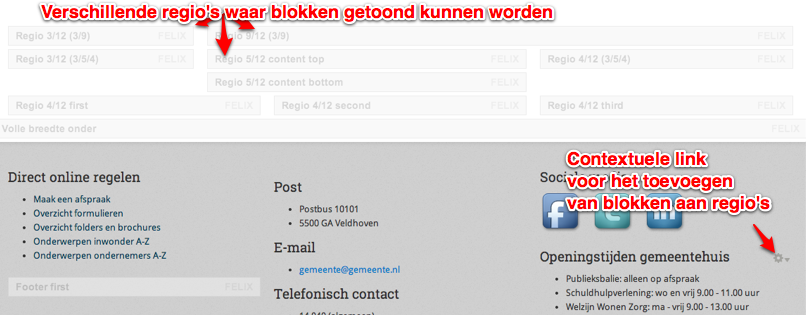
\includegraphics[width=\textwidth]{img/grid1.png}
\end{center}

\subsubsection{Blokken}

In het onderstaande afbeelding worden alle bestaande blokken op voorpagina in het kort toegelicht.

\bigskip

\begin{center}
	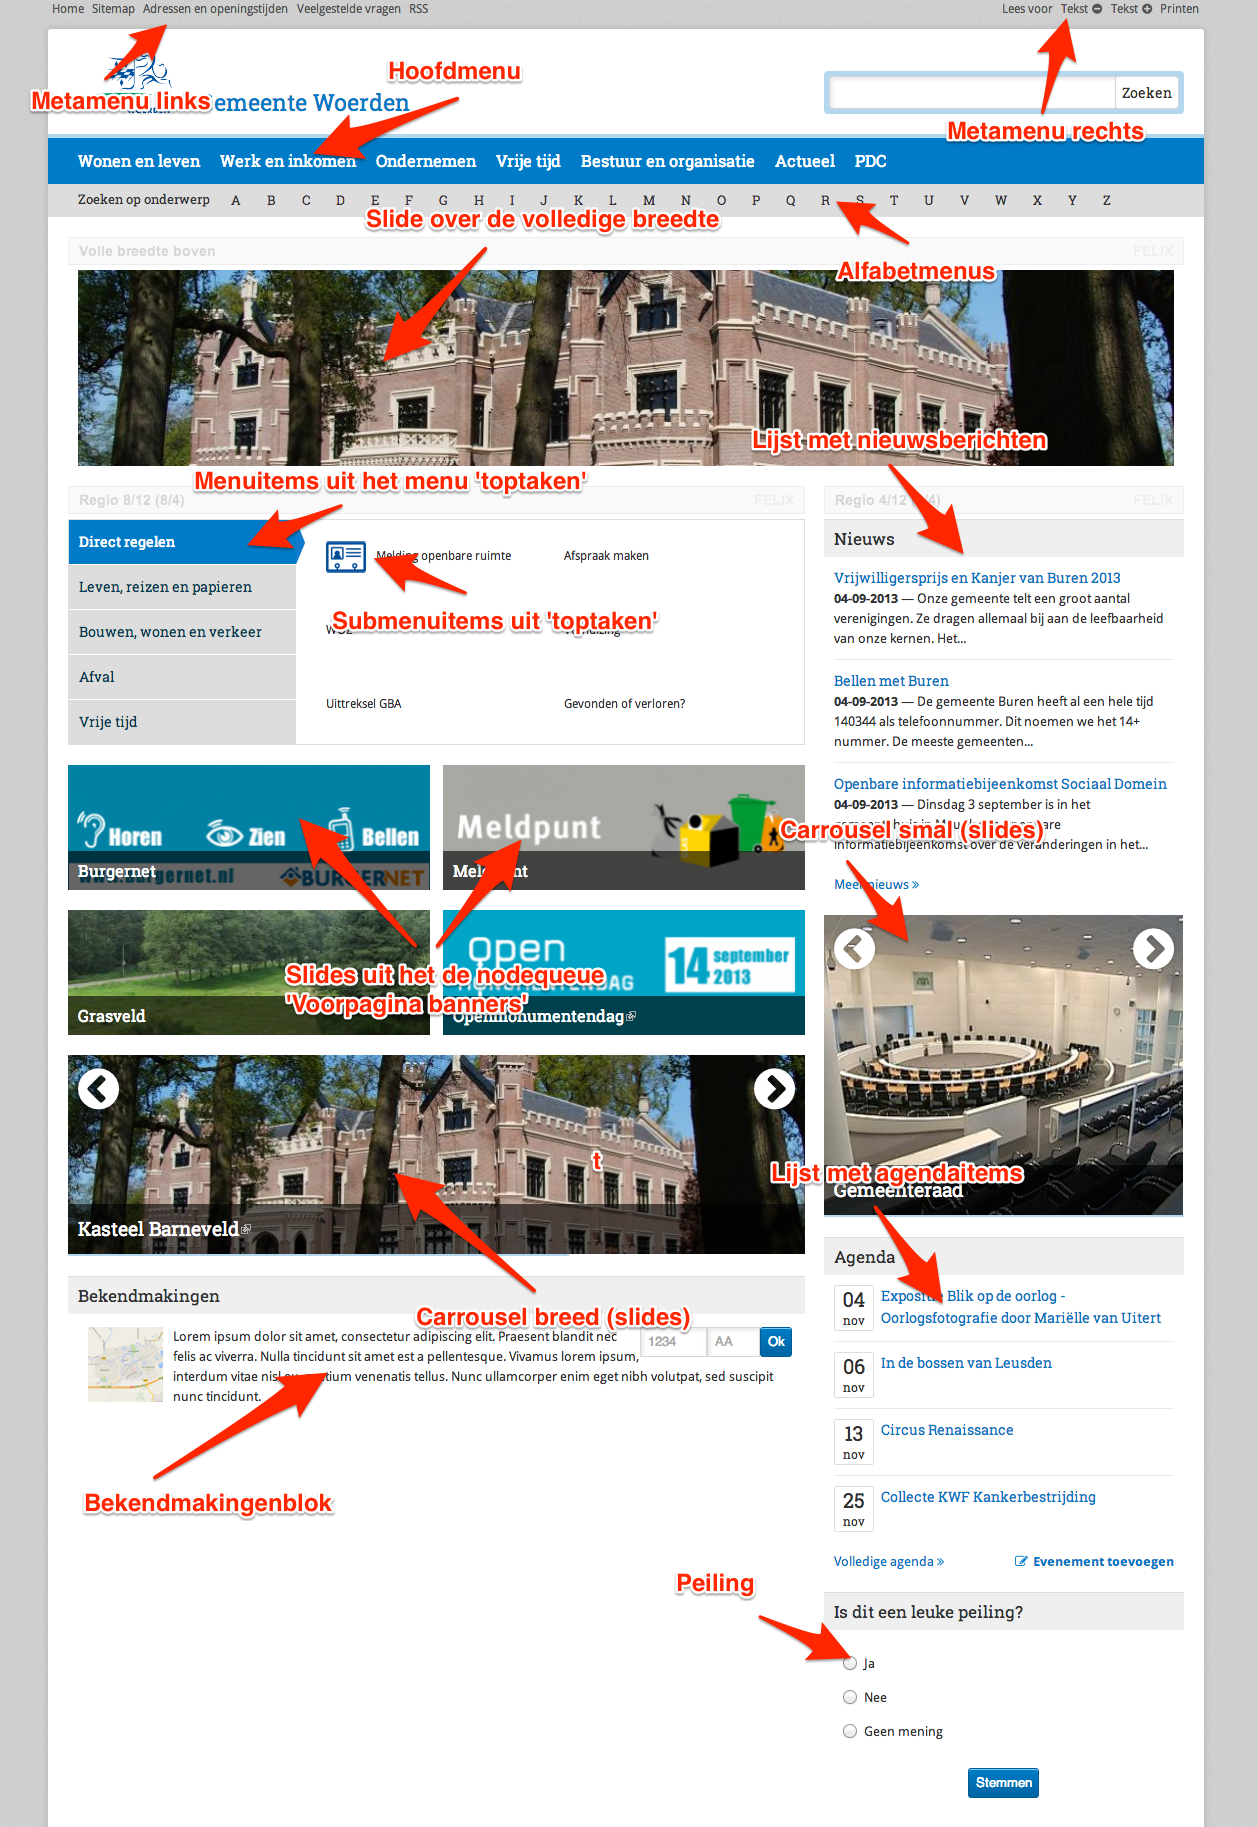
\includegraphics[width=\textwidth]{img/voorpagina.png}
\end{center}

\subsubsection{Footer}

In het onderstaande afbeelding worden alle bestaande blokken in de footer in het kort toegelicht. De footer bestaat uit 3 regio's waar blokken in gezet kunnen worden. De standaard configuratie is links een menu blok "Direct online regelen", in het hoofdstuk \emph{Menu}\seeone{menu} wordt beschreven hoe het menu te bewerken is. In de middenkolom staat blok met redactionele content. In de rechterkolom staan twee blokken; het eerste blok is het Dominion social blok. In paragraaf \emph{Social media}\seeone{socialmedia} staat beschreven hoe deze opties te beheren zijn. Daaronder staat nog een blok met redactionele content. Naast de standaard geconfigureerde blokken zijn in de drie regio's ook nog Felix blokken te zetten. 

\bigskip

\begin{center}
	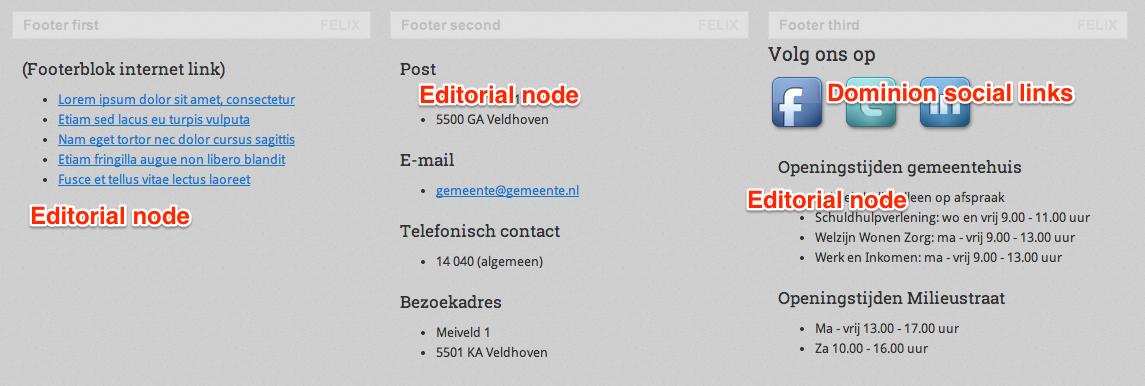
\includegraphics[width=\textwidth]{img/voorpagina3.png}
\end{center}
\subsection{Dashboard}\label{dashboard}
Het dashboard is de persoonlijke pagina voor ieder lid van het Intranet. Het is een pagina die is opgebouwd uit blokken die de gebruiker zelf kan aanzetten, uitzetten of verplaatsen.

In de onderstaande afbeelding zie je het Dashboard voor een Intranet gebruiker. 
Bij pijl 1 kun je blokken toevoegen aan je Dashboard. Elk blok heeft verschillende opties zoals inklappen, uitklappen en sluiten. Deze zijn te vinden bij pijl 2

\begin{center}
	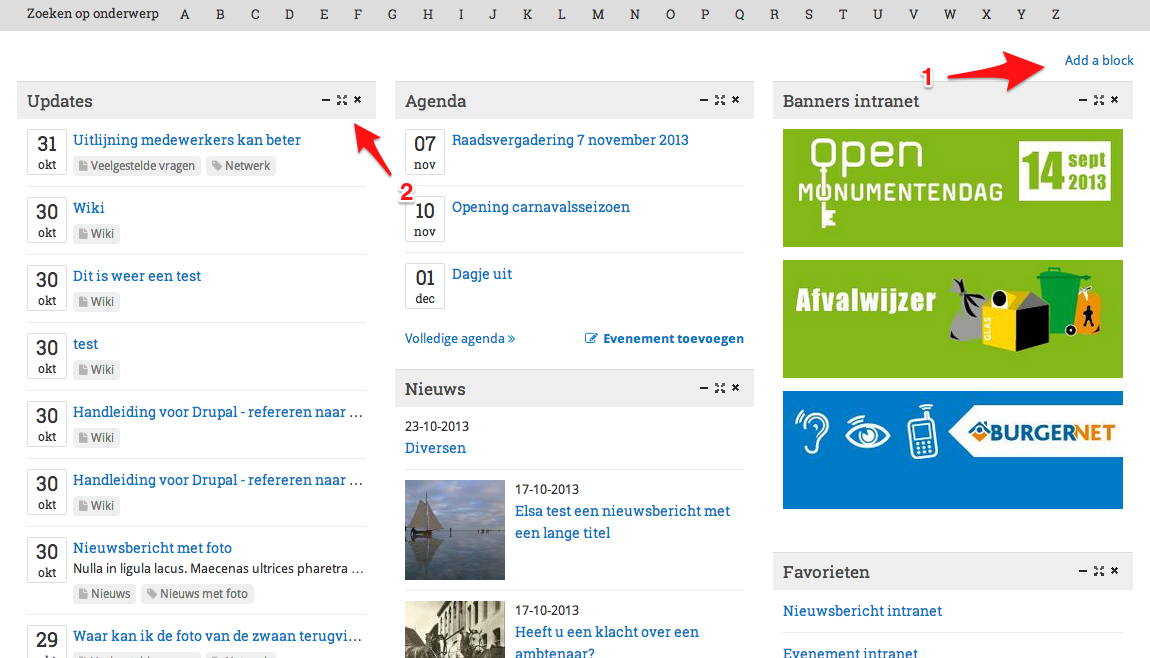
\includegraphics[width=\textwidth]{img/dashboard.png}
\end{center}

\subsection{Mobiel menu}

Op de mobiele versie verschijnt een blok met adres en telefoonnummer van het gemeentehuis. Dit blok is op een desktop browser ook te zien wanneer het scherm kleiner wordt gemaakt. Ingelogd als eindredacteur kan op deze manier ook de inhoud worden bewerkt op dezelfde manier als andere \emph{felix} blokken\seeone{felix}.


\section{Content management}\label{contentmanagement}

Het hoofdstuk �Content management� omschrijft alle relevante aspecten van het inhoudelijke beheer van de website.

\subsection{Workbench}\label{workbench}
De workbench biedt een handig overzicht voor (eind)redacteuren. Via de workbench kun je bijvoorbeeld makkelijk bekijken welke inhoud recentelijk is aangemaakt of welke inhoud nog beoordeeld moet worden.

\subsubsection{Workbench overview}\label{workbenchoverview}
De onderstaande afbeelding toont de Workbench. 
\bigskip

\begin{center}
	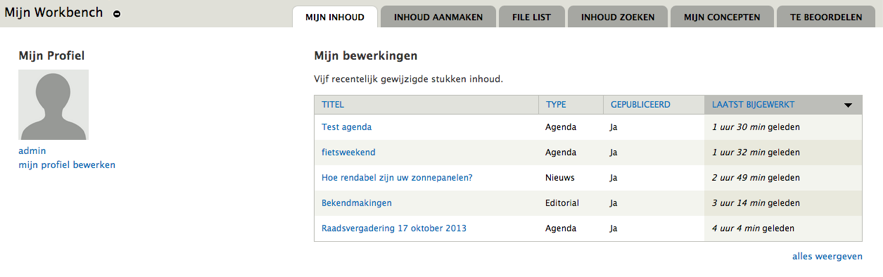
\includegraphics[width=\textwidth]{img/workbench.png}
\end{center}

\textbf{Mijn inhoud:} toont de inhoud welke recentelijk is bewerkt door de gebruiker.

\textbf{Inhoud toevoegen:} link naar de pagina \emph{Inhoud toevoegen}.

\textbf{File list:} toont alle bestanden welke recentelijk zijn toegevoegd.

\textbf{Inhoud zoeken:} link naar de pagina \emph{Inhoud zoeken}, hier kun je gemakkelijk met behulp van filters op inhoud zoeken.

\textbf{Mijn concepten:} toont alle concepten aangemaakt door de gebruiker.

\textbf{Te beoordelen:} toont alle content items welke nog goedgekeurd moeten worden door de eindredacteur.

\subsubsection{Workbench workflow}\label{workbenchworkflow}

De workflow binnen de workbench gaat als volgt. Een redacteur voert nieuwe content op als \emph{concept}. Zolang het een concept blijft zal deze terug te vinden zijn onder de tab \emph{Mijn concepten}. Dit item zal dan niet aan de voorkant te lezen zijn. De redacteur kan dan kiezen om het ter beoordeling aan te bieden. Het item zal dan verschijnen onder de tab \emph{Te beoordelen} van een gebruiker met de rol \emph{eindredacteur}. De eindredacteur kan dan kiezen om het item terug te zetten naar concept of om het te publiceren. 

Bij het bewerken van bestaande content geldt dezelfde flow. Van het bestaande item zal dan een nieuw concept gemaakt worden, wat door de redacteur ter beoordeling aangeboden kan worden. Om daarna door een eindredacteur te publiceren of terug te zetten naar concept.
\clearpage
\subsection{Workflow}\label{workflow}

In de website van \drupalpath wordt gebruik gemaakt van \emph{workflow}. Dat wil zeggen dat nieuwe inhoud en gewijzigde inhoud niet in alle gevallen direct op de site zal verschijnen, maar eerst goedgekeurd moet worden. Hierbij wordt onderscheid gemaakt tussen eindredacteuren en redacteuren. Eindredacteuren hebben het recht om content binnen de gehele website te publiceren en aan te passen. Eindredacteuren kunnen content van redacteuren tevens publiceren op andere delen van de site.

De workflow is zowel van toepassing op nieuwe als bestaande inhoud. Bij reeds bestaande inhoud wordt een nieuwe \emph{revisie} aangemaakt. De nieuwe revisie kan bestaan naast de gepubliceerde pagina. Zo is het mogelijk dat een wijziging pas later, na goedkeuring, gepubliceerd wordt en dus zichtbaar voor bezoekers.

Bij het invoeren of bewerken van content is onderin het formulier een item "Publicatie-opties\emph{ te zien. Hierin staat een item }Moderatie status". Daarin zitten de volgende opties:
\begin{itemize}
\item Mijn concepten
\item Te beoordelen
\item Gepubliceerd
\end{itemize}

Nieuwe inhoud of revisies worden als eerste aangemaakt als \emph{concept}. In deze staat is het een \emph{kladversie}. Bewerkingen hebben nog geen invloed op de website. Wanneer de content online mag dan kan de status op \emph{Te beoordelen} worden gezet. In deze staat krijgen eindredacteuren dit item te zien in een lijst met goed te keuren inhoud. Tevens wordt een mail gestuurd naar alle eindredacteuren. Het item kan daarna op \emph{Gepubliceerd} worden gezet. De inhoud wordt dan zichtbaar op de website voor alle bezoekers. Afhankelijk van de rechten is het mogelijk om in dit proces stappen over te slaan.


Onderstaand tabel toont de workflow per inhoudstype. 

\textbf{Gepubliceerd:} Na het opslaan wordt de content direct zichtbaar gemaakt op de website.

\textbf{Revisie:} Elke keer nadat een content item is bijgewerkt, wordt er een nieuwe revisie aangemaakt.

\textbf{Moderatie revisie:} Indien deze optie is geactiveerd, is het mogelijk een revisie te wijzigen.

\textbf{Ge{\"\i}mporteerd:} Content van dit inhoudstype zal ge{\"\i}mporteerd worden.

\textbf{J:} Ja (van toepassing).

\textbf{N:} Nee (niet van toepassing).

\begin{tabularx}{\textwidth}{ | p{5cm} |X|X|X|X| }
  \hline
  Inhoudstype & Gepubliceerd & Revisie & Moderatie revisie & Ge{\"\i}mporteerd \\ \hline
  Agenda & N & J  & J & N  \\ \hline
  Bekendmaking & N & J  & J & J  \\ \hline
  Bericht  & J & N  & N & N  \\ \hline
  Bestand  & J & N  & N & N  \\ \hline
  Bestemmingsplan  & J & N  & N & J  \\ \hline
  Blog  & J & N  & N & N  \\ \hline
  Editorial  & J & J  & N & N  \\ \hline
  Eenvoudige pagina  & N & J  & J & N  \\ \hline
  FAQ  & N & J  & J & N  \\ \hline
  Forumonderwerp  & J & N  & N & N  \\ \hline
  Foto  & J & N  & N & N  \\ \hline
  Marktplaats  & J & N  & N & N  \\ \hline
  Nieuws  & N & J  & J & N  \\ \hline
  Onderwerp  & J & N  & N & N  \\ \hline
  Peiling  & N & J  & J & N  \\ \hline
  Persoon  & N & J  & J & N  \\ \hline
  Product  & J & N  & N & J  \\ \hline
  RSS  & J & N  & N & J  \\ \hline
  RSS Source  & N & N  & N & N  \\ \hline
  Regeling  & J & N  & N & J  \\ \hline
  Slide  & N & J  & J & N  \\ \hline
  VAC  & J & N  & N & J  \\ \hline
  Webformulier  & J & N  & N & N  \\ \hline
  Wiki  & J & N  & N & N  \\ \hline
\end{tabularx}

\subsubsection{Revisies inzien en terugzetten}\label{modererentab}

De revisies van inhoud zijn later (ook na publicatie) terug te vinden onder het tabblad \emph{Modereren}. Op deze pagina is een lijst te zien waarin tevens de datum en workflow status te zien is. Met de link \emph{weergeven} kan de revisie worden bekeken. Met de link \emph{terugzetten} kan de revisie worden teruggezet. In het laatste geval publiceren we een oudere revisie, waarmee we alle latere wijzigingen ongedaan maken. Een revisie kan ook nieuwer zijn dan de versie die is gepubliceerd. In dit geval is er een \emph{publiceren} link aanwezig. Hiermee kan deze versie worden goedgekeurd en gepubliceerd.

Onder de link \emph{Vergelijk revisies} (2e niveau tabblad) zit een pagina waarmee makkeljik te verschillen tussen revisies zichtbaar gemaakt kunnen worden. Hierbij moeten twee revisies gekozen worden. Kies eerst de nieuwste revisie en daarna de oudere revisie (verder onderaan in de lijst). Klik daarna op de knop \emph{Vergelijken}. Hierna worden de tekstuele wijzigingen getoond. Dit heeft betrekking op de hoofdtekst van dit item.

\subsubsection{Inhoud goedkeuren}\label{inhoudgoedkeuren}

In het dashboard is voor eindredacteuren een lijst beschikbaar met inhoud dat goedgekeurd dient te worden. Dit is inhoud met de status \emph{Ter beoordeling}. Klik hiervoor linksboven op \emph{Mijn Workbench} en dan op \emph{Te beoordelen} (2e niveau tabblad). In deze lijst kan doorgeklikt worden naar de pagina's die goedgekeurd dienen te worden. Nadat de wijzigingen zijn bekeken kunnen deze worden goedgekeurd onder het tabblad \emph{Modereren}\seeone{modererentab}.

\begin{center}
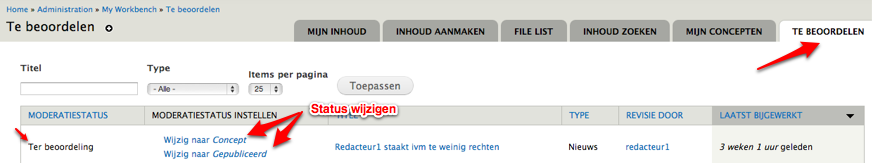
\includegraphics[width=\textwidth]{img/publiceren.png}
\end{center}
\subsection{Content beheer}\label{contentbeheer}
Alle content(inhoud) kan via de voorkant en de achterkant van de website beheerd worden. 
'Mijn Workbench' biedt een goede basis voor het beheren van content. Klik op 'Mijn Workbench' of ga direct naar \drupalpath{admin/workbench}. 

\subsubsection{Content toevoegen}\label{contenttoevoegen}
Algemene werkwijze voor het toevoegen van content:
\begin{enumerate}
\item Klik op de link 'Inhoud' of ga direct naar \drupalpath{node/add}.
\item Klik vervolgens op het gewenste inhoudstype, je zult nu het scherm te zien krijgen waarin je de daadwerkelijke content kunt toevoegen.
\item Vul alle verplichte velden in (velden met een (*)).
\item Vul desgewenst de optionele velden in.
\item Om de content op te slaan klik je onderaan de pagina op de knop 'Opslaan'.
\end{enumerate}

\bigskip

\begin{center}
	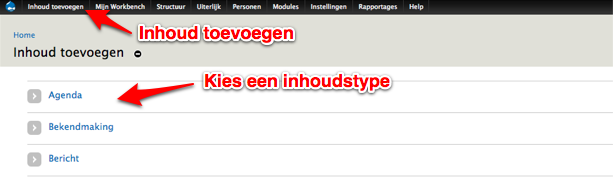
\includegraphics[width=\textwidth]{img/content1.png}
\end{center}

\subsubsection{Content bewerken}\label{contentbewerken}
Algemene werkwijze voor het bewerken van content:
\begin{enumerate}
\item Ga naar het overzicht van alle inhoud: \emph{Mijn Workbench} $\rightarrow$ \emph{Inhoud zoeken}, of ga direct naar \drupalpath{admin/workbench/all-content}.
\item Om de gewenste inhoud sneller te vinden kun je de filterfunctie gebruiken, bovenaan de pagina. Klik bijvoorbeeld bij het label 'type' in het lijstje op 'Agenda' en vervolgens klik je op 'Filteren'. Alleen artikelen van het type "Agenda" zullen nu getoond worden.
\item Zoek naar de titel van het artikel welke je wil gaan bewerken en klik vervolgens op 'bewerken' in de meest rechter kolom genaamd 'bewerken'.
\item Je bent nu gereed om de content te gaan bewerken. Om de bewerkingen op te slaan klik je onderaan de pagina op de knop 'Opslaan'.
\end{enumerate}

\begin{center}
	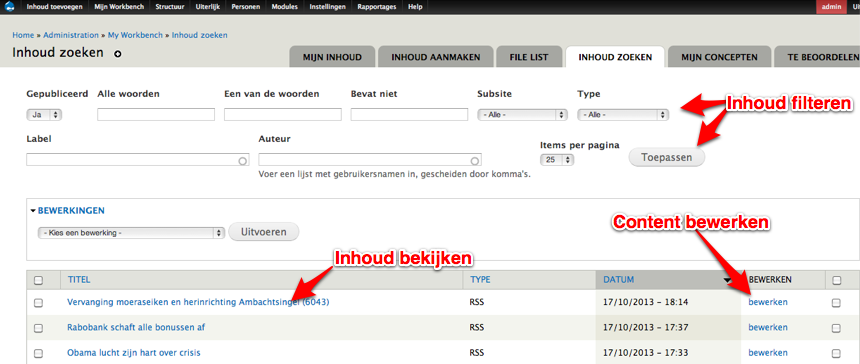
\includegraphics[width=\textwidth]{img/content2.png}
\end{center}

\subsubsection{Content verwijderen}\label{contentverwijderen}
Algemene werkwijze voor het verwijderen van content:
\begin{enumerate}
\item Ga naar het overzicht van alle inhoud: \emph{Mijn Workbench} $\rightarrow$ \emph{Inhoud zoeken}, of ga direct naar \drupalpath{admin/workbench/all-content}.
\item Om de gewenste inhoud sneller te vinden kun je de filterfunctie gebruiken, bovenaan de pagina. Klik bijvoorbeeld bij het label 'type' in het lijstje op 'Agenda' en vervolgens klik je op 'Filteren'. Alleen artikelen van het type "Agenda" zullen nu getoond worden.
\item Zoek naar de titel van het artikel welke je wil gaan bewerken en klik vervolgens op 'bewerken' in de meest rechter kolom genaamd 'bewerken'.
\item Onderaan de pagina staat de knop 'Verwijderen', klik op deze knop om de content te verwijderen. Na het bevestigen zal de content permanent en onherstelbaar verwijderd worden.
\end{enumerate}

\bigskip

\begin{center}
	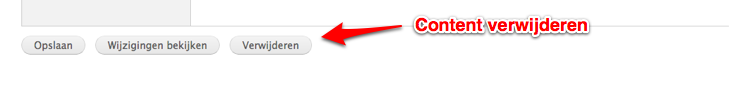
\includegraphics[width=\textwidth]{img/content3.png}
\end{center}
\subsection{Standaardvelden}
Alle content typen bevatten verschillende standaardvelden. De onderstaande lijst beschrijft elk veld apart.

\subsubsection{Titel}
De titel van de pagina, dit veld is altijd verplicht.

\subsubsection{Intro tekst}
De intro tekst van de pagina, dit veld is bij de meeste content typen niet verplicht. Deze tekst zal als introductie teaser worden getoond.

\subsubsection{Body tekst}
Dit veld is het meest belangrijk, in dit veld dient de hoofdtekst ingevuld te worden. Gebruik de editor om de tekst te stijlen met bijvoorbeeld vet gedrukte of cursieve teksten.

\subsubsection{Afbeeldingen}
Klik op �Selecteer media� bij het veld �Afbeeldingen�, selecteer een afbeelding en klik op �toevoegen�. Klik vervolgens op �Item toevoegen�. Herhaal deze stappen indien je meerdere afbeeldingen wil toevoegen.

\subsubsection{Media}\label{media}
\pvelist{ \pve{2.16} }
Klik op �Select media� bij het veld �Media�, selecteer een bestand en klik op �Indienen�. Indien je meerdere mediabestanden wilt toevoegen klik je op �Item toevoegen� en klik vervolgens op �Select media�.

Het is ook mogelijk om een video van het web toe te voegen. Klik op �Select media� bij het veld �Media�. Klik vervolgens op de tab �Web�. Bij het veld �URL or embed code� vul je de URL of embed code in. Dit is een voorbeeld URL om een youtube video toe te voegen:  \texttt{http://www.youtube.com/embed/Abiil-lD3HY} . Om het bestand toe te voegen klik je op �Indienen�.

Ook kan er een bestand uit de bibliotheek toegevoegd worden. Klik op �Select media� bij het veld �Media�. Klik vervolgens op de tab �Bibliotheek� en selecteer het gewenste bestand. Om het bestand toe te voegen klik je op �Indienen�. Toegestane bestandstypen zijn: �avi� (= video) en �mp3� (= audio).

\subsubsection{Attachments}
Klik op �Selecteer media� bij het veld �Attachments�, selecteer een bestand en klik op �toevoegen�. Klik vervolgens op �Item toevoegen�. Herhaal deze stappen indien je meerdere bestanden wil toevoegen.

\subsubsection{Tekstopmaak}
\pvelist { \pve{2.18} }
Onder het veld �Body� kan telkens gekozen worden tussen drie verschillende opties: �Filtered HTML�, �Full HTML� en �Plain text�.
\begin{itemize}
\item Filtered HTML: voorgedefinieerde HTML tags zullen worden toegestaan, alle overige HTML tags zullen uit de tekst gefilterd worden.
\item Full HTML: alle HTML tags zijn toegestaan.
\item Plain text:  alleen gewone tekst is toegestaan, alle HTML of andere code zal gefilterd worden zodra de pagina wordt opgeslagen.
\end{itemize}
Binnen \emph{Filtered HTML} is het mogelijk om \emph{iframes} toe te voegen. Dit zijn embedded webpagina's van andere websites. Deze kunnen worden gebruikt om 3th party modules zoals bijv. een enqu\^{e}te in te sluiten.

\subsubsection{Locatie}
Het locatieveld is beschikbaar in de volgende content types: Webformulier, Agenda, Bekendmaking, Bestemmingsplan, Pagina, Nieuws, Product. De veld bestaat uit twee onderdelen. Het eerste is het invullen van adres gegevens. Deze bestaat uit een locatienaam, de straat, de postcode, de woonplaats en het land. De waardes die hier ingevuld worden zullen gebruikt worden om de Google Maps link te genereren.

\begin{center}
	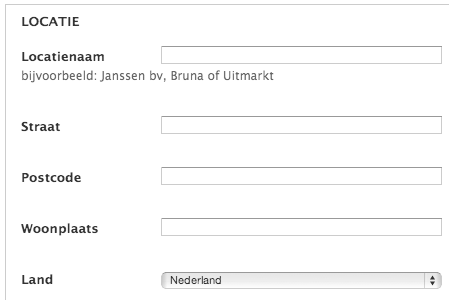
\includegraphics[width=\textwidth]{img/locatie1.png}
\end{center}

Het tweede deel van dit veld is een kaart met daaronder twee velden, Breedtegraad en Lengtegraad. Dit deel wordt gebruikt om het kaartje te tonen in de rechterkolom van een detailpagina. Er zijn twee manieren waarop een locatie aangegeven kan worden. Dat is door op de kaart te klikken en de pointer er neer te zetten. Of wanneer je de exacte breedte- en lengtegraad weet, deze in te vullen.

\begin{center}
	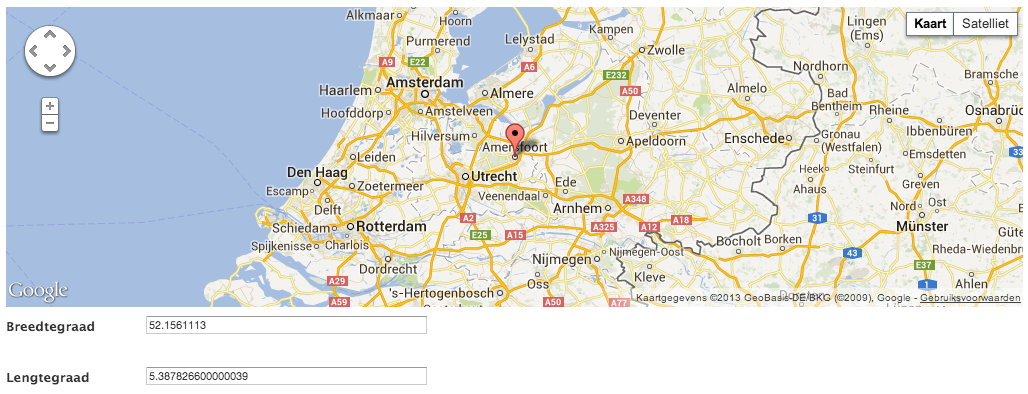
\includegraphics[width=\textwidth]{img/locatie2.png}
\end{center}

\subsubsection{URL alias}\label{alias}
\pvelist{ \pve{2.6}, \pve{2.6.1}, \pve{2.6.2} }
Nieuwe inhoud wordt automatisch op een vriendelijke URL geplaatst (bijv. \\ \texttt{\customerdomain /nieuws/2013/onderwerp}). Dit pad zal normaliter niet aangepast hoeven te worden. De \emph{URL alias} geeft het \emph{gebruikelijke} pad van de pagina weer. 

Het uitgangspunt is dat het automatische pad gehanteerd wordt, maar indien dit onwenselijke resultaten oplevert dan is het voor redacteuren wel mogelijk om dit pad aan te passen. Klik hiervoor bij het toevoegen of bewerken van inhoud op \emph{URL-pad-instellingen} (onderaan de pagina). Daar staat een checkbox die aangeeft dat er een automatische URL gebruikt wordt. Na het uitvinken hiervan kan eronder in een tekstveld een eigen pad worden aangegeven. 

Het is mogelijk om speciale tekens te gebruiken in de URL alias. Echter raden we het gebruik daarvan sterk af. In veel browsers worden deze getoond met een andere codering (een apostrof wordt bijvoorbeeld "\%E2\%80\%89"). Aanbevolen wordt om de tekens te beperken tot alfanumeriek (a t/m z en 0 t/m 9) en afbreekstreepjes. Het gebruik van hoofdletters is ook niet gebruikelijk in URL's.

\subsubsection{Publiceren onder embargo (Planneropties)}
Publiceren onder embargo is te vinden tussen de horizontale tabs bij het bewerken van een item. Het gaat om de tab \emph{Planneropties}.

Deze tab bevat een aantal datum/tijd velden.
\begin{itemize}
\item Publiceer revisie op \emph{(alleen bij bewerken)}
\item Publiceer op
\item Depubliceer op
\end{itemize}

Geen van de velden is verplicht en kunnen afzonderlijk van elkaar ingevuld worden. Wanneer alleen de \emph{Publiceer op} ingevuld wordt zal het item pas gepubliceerd worden na deze datum. Wanneer alleen \emph{Depubliceer op} ingevuld wordt zal het item na deze datum niet meer verschijnen. Worden beide velden ingevuld zal het item alleen tussen deze twee datums getoond worden.

De velden \emph{Publiceer op} en \emph{Depubliceer op} gaan over het (de)publiceren van de volledige node. Het is ook mogelijk om wijzigingen aan te brengen op een reeds gepubliceerd item, waarbij die wijzigingen op een bepaalde datum worden gepubliceerd. Daarvoor moet een datum worden ingevuld bij \emph{Publiceer revisie op}. De moderatie status onder \emph{Publicatie-opties} laat men in dat geval op \emph{Concept} staan, aangezien dat veld over de \emph{actuele} status gaat.

\subsection{Formulieren} \label{webform}
\pvelist{ \pve{4.24} }

\begin{enumerate}
\item Zorg ervoor dat u bent ingelogd en verzeker u ervan dat u de juiste rechten heeft om resultaten van webformulieren te bekijken.

\item Zoek het formulier op. Een webform is een node, dus u kunt bijvoorbeeld het content-overzicht gebruiken op admin/content en daar filteren op type \emph{Formulier}.

\item Ga naar het formulier en kies de tab \emph{Resultaten}. (Ziet u deze tab niet, dan heeft u onvoldoende rechten. Neemt u in dat geval contact op met uw systeembeheerder).

\item Kies de knop \emph{Downloaden} bovenaan het scherm.

\item Kies als export-formaat \emph{Karaktergescheiden tekst}. Dit biedt de meeste controle op het export-formaat. (De Excel-optie is beperkt en geeft geen werkelijk Excel-bestand).

\item Kies als scheidingsformaat \emph{Sluisteken (|)}. Dit is het meest universele teken, omdat de minste kans bestaat dat dit teken ook voorkomt in de data zelf.

\item Pasoptioneel de extra opties aan.

\item Klik op \emph{Download}.

\item Importeer het bestand in uw spreadsheet-programma (bijv. Excel). Verzeker u ervan dat de import-instellingen juist staan, met name dat ook hier het scheidingskarakter op het pipe-symbool (|) staat.
\end{enumerate}

\subsubsection{Formulieren valideren}
Er zijn regels gemaakt om te valideren wat de gebruiker heeft ingevoerd in het formulier. Deze regels zijn te wijzigen onder het tabblad \emph{Webform} $\Rightarrow$ \emph{Form validation}.

\begin{center}
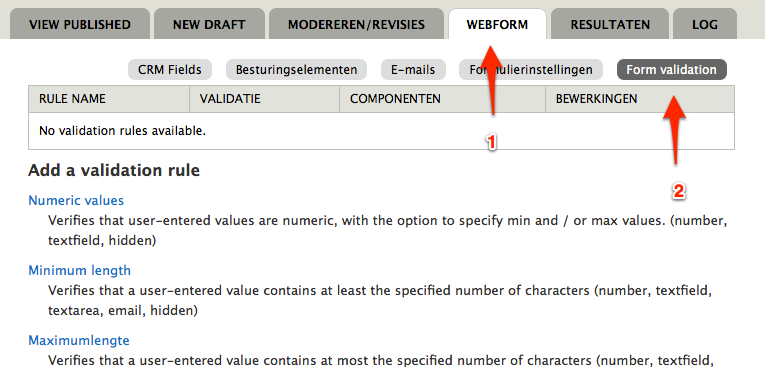
\includegraphics[width=\textwidth]{img/formvalidation.png}
\end{center}

Op deze pagina staat een heel scala aan opties. De volgende zijn met name relevant:
\begin{itemize}
\item Equal values \\
Controleert of de waarde van een veld overeenkomt met de waarde van een ander veld. Dit kan worden gebruikt voor een extra controle op bijv. e-mailadres. Hierbij worden twee e-mail velden aangemaakt. Daarna kan deze regel worden toegevoegt. De regel moet altijd een naam hebben, bijv. "emailcheck" (deze wordt niet getoont aan de gebruiker). Vink daarna de velden aan die gelijk moeten zijn.
\item Regular expression, case insensitive \\
Kan voor diverse doeleinden worden gebruikt. Reguliere expressies zijn een aparte taal dat specifiek voor validatie is bedoeld. Zie verder voor voorbeelden.
\item Regular expression, case sensitive \\
Idem, maar dan hoofdletter gevoelig.
\end{itemize}
Bij de reguliere expressies moeten de volgende gegevens worden opgegeven:
\begin{itemize}
\item Naam, bijv. "postcodecheck" (deze wordt niet getoont aan de gebruiker)
\item Velden waarop de validatie van toepassing is (aanvinken)
\item Regex code (zie verder)
\item Aangepaste foutmelding, bijv. "De postcode is onjuist."
\item Negate rule: vink deze aan om de regel om te draaien ("mag niet voldoen aan"). In de praktijk wordt deze zelden gebruikt.
\end{itemize}
De regex code bepaald welke invoer valide is. Deze kunnen direct overgenomen worden van de volgende voorbeelden:
\begin{verbatim}
Postcode (Nederlands, met spatie):       ^[1-9][0-9]{3} [A-Z]{2}$
Postcode (Nederlands, zonder spatie):    ^[1-9][0-9]{3}[A-Z]{2}$
Postcode (Nederlands, spatie optioneel): ^[1-9][0-9]{3} ?[A-Z]{2}$
Telefoon (Nederlands vast):              ^0[^6]{1,2}[0-9 \-]{7,10}$
Telefoon (Nederlands mobiel):            ^06[ \-]?[0-9]{8}$
Telefoon (Nederlands mobiel of vast):    ^0[0-9]{1,3}[0-9 \-]{8,10}$
Huisnummer:                              ^[1-9][0-9]* ?[a-z]{,5}.?[0-9]*$
\end{verbatim}
Enkel het stuk van \texttt{\^} t/m \texttt{\$} dient overgenomen te worden.

Voor het valideren van een e-mailadres wordt geen reguliere expressie gebruikt. Er is een type "email" dat gebruikt kan worden als veldtype waar automatisch de goede validatie inzit.

Voor valideren van internationele postcodes is geen reguliere expressie beschikbaar omdat er internationaal geen vast patroon is waar deze aan voldoen. Bij huisnummers moet erop worden gelet dat er uitzonderingen zijn voor bijv. woonboten waarbij "t/o museum" als geldig huisnummer aangemerkt dient te worden. De reguliere expressie houd geen rekening met deze uitzonderingen. Het huisnummer moet hierbij altijd beginnen met tenminste \'{e}\'{e}n cijfer (hoger dan 0), eventueel gevolgd door een letter en evt. weer een cijfer (waarbij spaties gebruikt mogen worden).

Op internet zijn talloze voorbeelden van reguliere expressies te vinden. De site \texttt{regexlib.com} bevat een uitgebreide bibliotheek. Ook via Google zijn deze makkelijk te vinden. Echter zijn er wel meerdere 'dialecten'. In Drupal wordt het "Perl" dialect gebruikt (de term "perl compatible" kom je hier weleens tegen). Dit is het meestgebruikte dialect, maar goed testen is altijd van belang!

\subsubsection{Bedankttekst}
Op \drupalpath{node/86/webform/configure} kan een bedankttekst geplaatst worden.

%todo: screenshots

\subsubsection{Verborgen veld}
Bij het aanmaken van een Formulier, kun je nu een veld toevoegen dat niet zichtbaar is aan de voorkant. Dit doe je door te kiezen voor type \emph{Verborgen} en de tekst van \emph{sleutelveld} te laten beginnen met een underscore  

\begin{center}
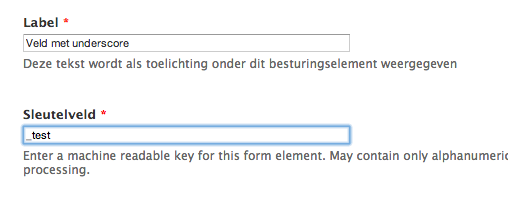
\includegraphics[width=\textwidth]{img/verborgenveld1.png}
\end{center}
Je kunt deze velden nu ook invullen als ingelogde gebruiker in het 'gewone' formulier.

Als je dus een besturingselement hebt toegevoegd waarvan het sleutelveld begint met een underscore, zie je dit veld staan bij de inzendingen in de backend

\begin{center}
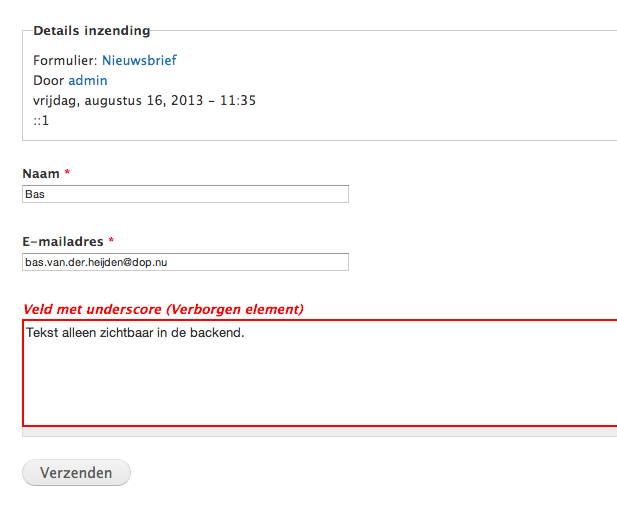
\includegraphics[width=\textwidth]{img/verborgenveld2.png}
\end{center}

\subsection{Formulieren importeren via CSV}

Het is mogelijk om resultaten van een formulier in CSV formaat in 1 keer te uploaden. Hierbij is het tevens mogelijk om (bijvoorbeeld bij de Nieuwsbrief formulieren) de bevestiging direct op \textbf{Ja} te zetten. Als je resultaten van een formulier op deze manier invult, worden er \textbf{geen} e-mails verstuurd.

Je begint het proces door naar de resultaten van een Formulier te navigeren, en daar te klikken op \textbf{Uploaden}.

\subsubsection{Template downloaden}

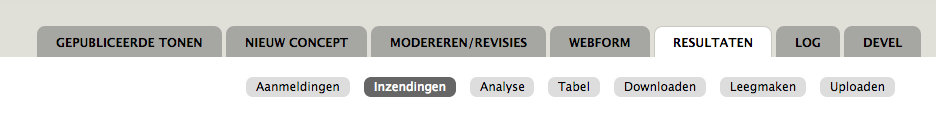
\includegraphics[width=\textwidth]{img/webform-upload.png}

Het is de bedoeling dat je eerst een template download van de vereiste CSV opmaak. Zo weet je namelijk zeker dat het CSV bestand dat je wilt uploaden, overeenkomt met de veld definities van het betreffende formulier. Als je al een CSV bestand hebt waar data in staat die je wilt uploaden, kun je deze het beste knippen/plakken naar het te downloaden template bestand. Dit voorkomt mogelijke fouten.

Je download een template door te klikken op een van de twee \textbf{Download Template} knoppen.

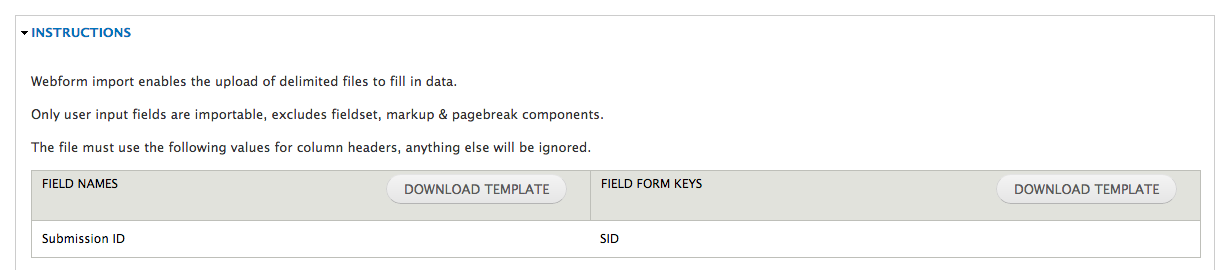
\includegraphics[width=\textwidth]{img/webform-template.png}

Het maakt niet uit welke van de twee beschikbare knoppen je kiest, maar het is wel belangrijk dat je later bij het uploaden van je data onder het kopje \textbf{Column header contains} dezelfde waarde kiest, respectievelijk \textbf{Field Form Keys} of \textbf{Field Names}.

Let ook op de dikgedrukte velden die in de tabel staan onder de \textbf{Download Template} knop. Deze velden zijn verplicht, en kun je dus niet leeg laten in het CSV bestand dat je later zult uploaden.
Velden die niet dikgedrukt zijn, kun je in het CSV bestand leeg laten. Deze velden worden dan bij de resultaten niet ingevuld. Wel is het belangrijk dat de koppen alsnog in het CSV bestand terugkomen, om een goede mapping te garanderen. Als je een verplicht veld graag leeg wilt laten, kun je de betreffende component tijdelijk op niet verplicht zetten, de resultaten uploaden en later weer verplicht maken.

Na het downloaden van het template bestand, kun je deze importeren in het Excel bestand waar je data in staat. Dit doe je door in (de Nederlandse versie van) Excel te kiezen voor \textbf{Gegevens} -> \textbf{Verbinden} en het gedownloade bestand te selecteren. Je kiest vervolgens voor type \textbf{Gescheiden} en \textbf{Puntkomma}. 

\subsubsection{Resultaten uploaden}

Let er bij het maken van het CSV bestand op dat alle waarden voor velden van type \textbf{Keuzelijst} overeen moeten komen met de titel, en dus niet de machine waarde. Voorbeeld: vul bij aanhef in het CSV bestand 'Dhr.' in, en niet 'm'.

Bij het uploaden van het CSV bestand is het belangrijk om de file delimiter op \textbf{Puntkomma} te zetten, gelijk aan het template dat je hebt gedownload. Je kunt controleren of jouw CSV bestand hieraan voldoet, door deze te openen met Notepad en te kijken of de waarden die ingevuld zijn, gescheiden zijn door een komma (,).

Kies vervolgens de juiste waarde voor de optie \textbf{Column header contains}, selecteer het bestand en klik op \textbf{Verzenden}. De waarden zijn nu ingevuld.
\subsection{Wysiwyg en media}\label{wysiwyg}

Voor media en wysiwyg worden de \usemodule{wysiwyg} en \usemodule{media} / \usemodule{file\_entity} modules ingezet. Als editor zelf wordt gekozen voor \texttt{CKEditor} aangezien dit de meestgebruikte editor is binnen Drupal en standaard is in Drupal 8.

\subsubsection{Buttons}

De buttons staan gespecificeerd in het FO document.
Een aantal buttons zit niet standaard in de \usemodule{wysiwyg} module. Hiervoor wordt de reeds ontwikkelde \texttt{ckeditor\_customtags} module gebruikt waarmee buttons kunnen worden toegevoegd.

\subsubsection{Links in bodytekst}

Voor het gemakkelijk kunnen toevoegen van links in bodyteksten wordt gebruik gemaakt van de \usemodule{linkit} module i.c.m. \usemodule{pathologic}.

\subsubsection{Invoerformaten}\label{invoerformaten}

Er worden drie invoerformaten ter beschikking gesteld voor gebruikers en redacteuren.

\begin{itemize}
\item \textbf{Full HTML} \\
Volledige HTML zonder filtering. Alleen beschikbaar voor eindredacteuren. Het wordt aanbevolen om hier spaarzaam gebruik van te maken vanwege de mogelijkheid om nieuwe XSS issues (security issues) te introduceren.
\item \textbf{Filtered HTML} \\
Standaard filtering op ongewenste HTML en herschrijven van links door \texttt{pathologic}.
\item \textbf{Plain text} \\
Wordt gebruikt voor reviews (geplaatst door bezoekers). Hierbij wordt geen opmaak / HTML toegestaan.
\end{itemize}

\subsubsection{Media}\label{media}

Images en video's moeten toegevoegd en hergebruikt kunnen worden in wysiwyg en bestandsvelden.
Uitgangspunt is versie 2 van de \texttt{media} module.



\subsection{Tabs toevoegen}\label{tabstoevoegen}
Aan alle inhoudstypen kunnen "Tabs" toegevoegd worden. 
Tabs toevoegen kan alleen bij velden waarbij de WYSIWYG editor geactiveerd is; op het veld "Body" is vrijwel altijd de WYSIWYG editor geactiveerd.

Een tab moet opgebouwd worden uit twee delen: de titel van de tab en de content van de tab.

\textbf{Een tab toevoegen:} 

\begin{enumerate}
\item Vul twee asterisken in (**), gevold door een spatie en vul vervolgens de titel van de tab in (** Tab1).
\item Selecteer met je muis de hele regel (zie screenshot).
\item Maak van deze selectie een \emph{H2} (heading 2).
\item Druk op de enter toets om naar de volgende regel toe te gaan, vul hier de inhoud van de tab in.
\item Herhaal deze stappen indien je meerdere tabs wil toevoegen.
\end{enumerate}

De onderstaande screenshot toont visueel aan hoe je tabs kunt toevoegen.

\begin{center}
	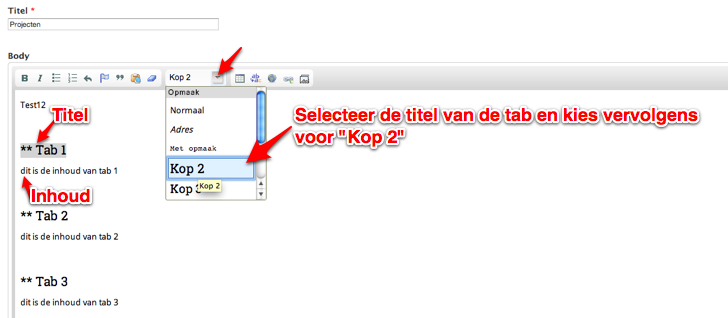
\includegraphics[width=\textwidth]{img/tabs1}
\end{center}

De onderstaande screenshot toont het resultaat.

\begin{center}
	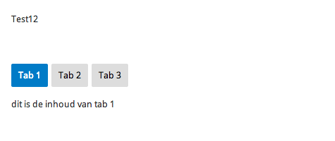
\includegraphics[width=\textwidth]{img/tabs2}
\end{center}
\subsection{Inhoudstypen}\label{inhoudstypen}
Inhoudstypen worden gebruikt voor het weergeven van verschillende typen inhoud. Per inhoudstype kunnen bijvoorbeeld verschillende velden gedefinieerd worden en de bijbehorende pagina's kunnen apart gestijled worden. Het gebruik van inhoudstypen cre�ert veel flexibiliteit.

In de volgende paragraaf zullen specifieke inhoudstypen nader beschreven worden.

\subsubsection{Agenda}\label{agenda}

\begin{enumerate}
\item Vul een titel in bij het veld 'Titel'.
\item Vul optioneel een introductie tekst in bij het veld 'Intro'.
\item Vul de hoofdtekst in bij het veld 'Body'.
\item Upload optioneel een afbeelding bij het veld 'Image'.
\item Specificeer optioneel een (eind)datum - kruis 'toon einddatum' aan om een einddatum te specificeren.
\item Specificeer optioneel een datum en tijd (bijvoorbeeld wanneer een evenement start) bij het veld 'Datum'.
\item Specificeer optioneel een locatie bij de velden onder 'Locatie'.
\item Voeg optioneel de content toe aan de kalender, dit doe je d.m.v. een datum te specificeren bij het veld 'Datum'.
\item Klik onderaan de pagina op de knop 'Opslaan' om de inhoud op te slaan.
\end{enumerate}

\subsubsection{Bekendmaking}\label{bekendmaking}

\begin{enumerate}
\item Vul een titel in bij het veld 'Titel'.
\item Selecteer het type bekendmaking.
\item Voeg optioneel de content toe aan de kalender, dit doe je d.m.v. een datum te specificeren bij het veld 'Datum'.
\item Vul de hoofdtekst in bij het veld 'Body'.
\item Specificeer optioneel een locatie bij de velden onder 'Locatie'.
\item Klik onderaan de pagina op de knop 'Opslaan' om de inhoud op te slaan.
\end{enumerate}

\subsubsection{Bericht}\label{bericht}

\begin{enumerate}
\item Vul een titel in bij het veld 'Titel'.
\item Vul de hoofdtekst in bij het veld 'Body'.
\item Klik onderaan de pagina op de knop 'Opslaan' om de inhoud op te slaan.
\end{enumerate}

\subsubsection{Bestand}\label{bestand}

\begin{enumerate}
\item Vul een titel in bij het veld 'Titel'.
\item Upload het gewenste bestand bij het veld 'Bestand'.
\item Klik onderaan de pagina op de knop 'Opslaan' om de inhoud op te slaan.
\end{enumerate}

\subsubsection{Bestemmingsplan}\label{bestemmingsplan}

\begin{enumerate}
\item Vul een titel in bij het veld 'Titel'.
\item Selecteer het type en de status van het bestemmingsplan bij de velden 'Type' en 'Status'
\item Voeg eventueel links toe naar documenten bij de velden 'Regels', 'Beleids document', 'Besluits document', 'Toelichting', 'Vastellings besluit', 'Bijlage' en/of 'Illustratie'. Vul een titel in en een url en klik op de knop 'Item toevoegen'. Herhaal deze stappen om meerdere links toe te voegen. 
\item Specificeer optioneel een locatie bij de velden onder 'Locatie'.
\item Klik onderaan de pagina op de knop 'Opslaan' om de inhoud op te slaan.
\end{enumerate}

\subsubsection{Blog}\label{blog}

\begin{enumerate}
\item Vul een titel in bij het veld 'Titel'
\item Upload optioneel een afbeelding bij het veld 'Image'
\item Vul optioneel een introductie tekst in bij het veld 'Intro'
\item Vul de hoofdtekst in bij het veld 'Body'.
\item Vul eventueel tags in, gescheiden met een spatie.
\item Klik onderaan de pagina op de knop 'Opslaan' om de inhoud op te slaan.
\end{enumerate}

\subsubsection{Editorial}\label{editorial}

\begin{enumerate}
\item Vul een titel in bij het veld 'Titel'
\item Vul de hoofdtekst in bij het veld 'Body'.
\item Klik onderaan de pagina op de knop 'Opslaan' om de inhoud op te slaan.
\end{enumerate}

\subsubsection{Eenvoudige pagina}\label{eenvoudigepagina}

\begin{enumerate}
\item Vul een titel in bij het veld 'Titel'.
\item Vul de hoofdtekst in bij het veld 'Body'.
\item Specificeer optioneel een locatie bij de velden onder 'Locatie'.
\item Klik onderaan de pagina op de knop 'Opslaan' om de inhoud op te slaan.
\end{enumerate}

\subsubsection{FAQ}\label{faq}

\begin{enumerate}
\item Vul een titel(vraag) in bij het veld 'Titel'.
\item Vul de hoofdtekst(antwoord) in bij het veld 'Body'.
\item Selecteer een FAQ Categorie bij het veld 'Categorie'.
\item Klik onderaan de pagina op de knop 'Opslaan' om de inhoud op te slaan.
\end{enumerate}

\subsubsection{Forumonderwerp}\label{forumonderwerp}

\begin{enumerate}
\item Vul een onderwerp in bij het veld 'Onderwerp'.
\item Selecteer een Forum Categorie bij het veld 'Forums'.
\item Vul de hoofdtekst in bij het veld 'Body'.
\item Klik onderaan de pagina op de knop 'Opslaan' om de inhoud op te slaan.
\end{enumerate}

\subsubsection{Foto}\label{foto}

\begin{enumerate}
\item Vul een titel in bij het veld 'Titel'.
\item Vul eventueel de hoofdtekst(uitgebreide foto omschrijving) in bij het veld 'Body'.
\item Upload een foto bij het veld 'Foto'.
\item Vul minstens 1 tag in bij het veld 'Tags', scheid meerdere tags met een spatie
\item Klik onderaan de pagina op de knop 'Opslaan' om de inhoud op te slaan.
\end{enumerate}

\subsubsection{Marktplaats}\label{marktplaats}

\begin{enumerate}
\item Vul een titel in bij het veld 'Titel'.
\item Vul eventueel een intro in bij het veld 'Intro'
\item Vul de hoofdtekst in bij het veld 'Body'.
\item Selecteer een categorie(aangeboden of gevraagd) bij het veld 'Categorie'.
\item Klik onderaan de pagina op de knop 'Opslaan' om de inhoud op te slaan.
\end{enumerate}

\subsubsection{Nieuws}\label{nieuws}

\begin{enumerate}
\item Vul een titel in bij het veld 'Titel'.
\item Vul eventueel een intro in bij het veld 'Intro'
\item Vul de hoofdtekst in bij het veld 'Body'.
\item Upload optioneel een afbeelding bij het veld 'Image'.
\item Vul eventueel tags in, gescheiden met een spatie.
\item Specificeer optioneel een locatie bij de velden onder 'Locatie'.
\item Klik onderaan de pagina op de knop 'Opslaan' om de inhoud op te slaan.
\end{enumerate}

\subsubsection{Onderwerp}\label{onderwerp}

\begin{enumerate}
\item Vul een titel in bij het veld 'Titel'.
\item Vul de hoofdtekst in bij het veld 'Body'.
\item Klik onderaan de pagina op de knop 'Opslaan' om de inhoud op te slaan.
\end{enumerate}

\subsubsection{Peiling}\label{peiling}

\begin{enumerate}
\item Vul een vraag in bij het veld 'Vraag'.
\item Vul minstens twee mogelijke antwoorden in bij het veld 'Keuze', klik op de knop 'Meer keuzes' om meerdere keuzes te specificeren.
\item Bepaal bij het veld 'Peilingsstatus' of de Peiling 'gesloten' of 'actief' is.
\item Selecteer hoe lang de Peiling moet duren bij het veld 'Peilingsduur'.
\item Specificeer optioneel een locatie bij de velden onder 'Locatie'.
\item Klik onderaan de pagina op de knop 'Opslaan' om de inhoud op te slaan.
\end{enumerate}

\subsubsection{Persoon}\label{persoon}

\begin{enumerate}
\item Vul een titel in bij het veld 'Titel'.
\item Upload optioneel een afbeelding bij het veld 'Image'.
\item Selecteer minstens 1 categorie bij het veld 'Category'.
\item Vul de hoofdtekst in bij het veld 'Body'.
\item Klik onderaan de pagina op de knop 'Opslaan' om de inhoud op te slaan.
\end{enumerate}

\subsubsection{Product}\label{product}

\begin{enumerate}
\item Vul een titel in bij het veld 'Titel'.
\item Vul een tekst in bij het veld 'Aanvraag', 'Beschrijving', 'Contact', 'Bezwaar', 'Kosten', 'Bijzonderheden' en 'Termijn'
\item Specificeer optioneel een locatie bij de velden onder 'Locatie'.
\item Maak 'Tabbed content' aan bij het veld 'Tabcontent'. Om meerdere tabs toe te voegen klik je op de knop 'Item toevoegen' onder het veld 'Tabcontent'.
\item Klik onderaan de pagina op de knop 'Opslaan' om de inhoud op te slaan.
\end{enumerate}

\subsubsection{RSS}\label{rss}
RSS Feed items worden automatisch ge�mporteerd. 

\subsubsection{RSS Source}\label{rsssource}
Met een 'RSS Source' kun je een uit een bron RSS Feeds ophalen.

\begin{enumerate}
\item Vul een titel in bij het veld 'Titel'.
\item Vul een URL in bij het veld 'URL'. Let op: de feed zal niet werken als de URL foutief is ingevuld.
\item Vul eventueel een hoofdtekst in bij het veld 'Body'.
\item Klik onderaan de pagina op de knop 'Opslaan' om de inhoud op te slaan.
\end{enumerate}

\subsubsection{Regeling}\label{regeling}
Regelingen worden automatisch ge�mporteerd.

\subsubsection{Slide}\label{slide}

\begin{enumerate}
\item Vul een titel in bij het veld 'Titel'.
\item Vul eventueel een URL in bij het veld 'Link', de 'Slide' zal doorlinken naar de opgegeven URL.
\item Upload een afbeelding bij het veld 'Image'.
\item Vul eventueel een hoofdtekst in bij het veld 'Body'.
\item Klik onderaan de pagina op de knop 'Opslaan' om de inhoud op te slaan.
\end{enumerate}

\subsubsection{VAC}\label{vac}

\begin{enumerate}
\item Vul een titel in bij het veld 'Titel'.
\item Vul een antwoord in bij het veld 'Antwoord'.
\item Vul een toelichting in bij het veld 'Toelichting'.
\item Klik onderaan de pagina op de knop 'Opslaan' om de inhoud op te slaan.
\end{enumerate}

\subsubsection{Wiki}\label{wiki}
Het inhoudstype 'wiki' zal worden gebruikt voor het aanmaken van informatieve pagina's.

Om een wiki pagina aan te maken ga je naar: \emph{Inhoud toevoegen} $\rightarrow$ \emph{Wiki} , of ga direct naar \drupalpath{node/add/wiki}.

Vul een titel bij het veld 'Titel' en vul informatieve tekst in bij het veld 'Body'.

Voor het inhoudstype 'Wiki' is een speciale filter gebouwd, deze filter maakt het refereren naar andere wiki pagina's mogelijk. 

Het refereren naar een andere wiki pagina gaat als volgt: 

\begin{enumerate}
\item Kopieer de titel van de node waarnaar je wilt refereren, bijvoorbeeld 'wiki pagina'
\item In de body tekst van je huidige node kun je refereren naar de node 'wiki pagina'
\item Plaats de node waarnaar je wilt refereren tussen dubbele 'square brackets': [[wiki pagina]]
\item Bijvoorbeeld: dit is informatie, op de pagina [[wiki pagina]] kun je meer informatie vinden.
\end{enumerate}

\bigskip

\begin{center}
	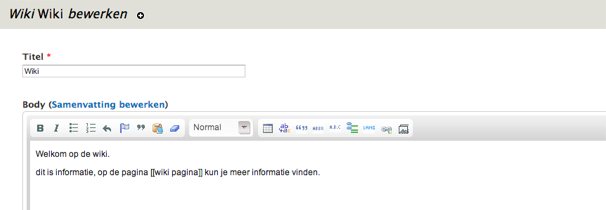
\includegraphics[width=\textwidth]{img/wiki.png}
\end{center}
\subsection{Nodequeues}\label{nodequeues}
Nodequeues zijn kort omschreven: \emph{wachtrijen voor content items (nodes)}. In een nodequeue kun je precies bepalen welke content er weergegeven wordt, het aantal en de volgorde van de toegevoegde content items.

\subsubsection{Nodequeues aanmaken}
Klik op de link �Structuur� en klik vervolgens op �Nodequeues� of ga direct naar \drupalpath{admin/structure/nodequeue}. Bovenaan de pagina verschijnen twee links: �exams queue toevoegen� en �simple queue toevoegen�.
Klik op �simple queue toevoegen� om een nodequeue aan te maken.

Je zult nu op de pagina terecht komen waar je een nieuwe queue kunt toevoegen.
\begin{enumerate}
\item Vul een titel in om de wachtrij een naam te geven
\item Limiteer hoeveel content items er kunnen worden getoond in de wachtrij, vul �0� (nul) in voor een onbeperkt aantal.
Kruis het vakje aan bij �Reverse in admin view� indien je content items vooraan de wachtrij wil toevoegen i.p.v. achteraan de wachtrij. 
\item Sla de stappen bij de velden �Link �add to queue� en �remove from queue� text� over.
\item Kruis aan bij �Rollen� welke gebruikers content items aan de nodequeue kunnen toevoegen.
\item Kruis aan bij �Typen� welke content items behorende bij de content typen toegevoegd kunnen worden aan de nodequeue.
\end{enumerate}

\subsubsection{Content toevoegen aan nodequeues}

Klik op de link �Structuur� en klik vervolgens op �Nodequeues� of ga direct naar \drupalpath{admin/structure/nodequeue}. Indien je al nodequeues hebt aangemaakt zal op deze pagina een lijst geladen worden met alle aangemaakte nodequeues. Klik op �Weergeven� in de meest rechter kolom om de wachtrij te tonen met alle toegevoegde content items. 

In het veld welke gevuld is met de tekst �Enter the title of a node to add it to the nodequeue�, vul je (deels) de titel in van het content item dat je aan de wachtrij wilt toevoegen. De titel hoef je slechts deels in te vullen omdat de website de titel automatisch zal aanvullen (indien de titel bestaat). Klik op de gevonden titel en klik vervolgens op �Inhoud toevoegen�.

Herhaal deze stappen om meerdere content items aan de nodequeue toe te voegen. Vervolgens kun je alle content items sorteren: handmatig, met de knop �omkeren� of �shuffle�.
\begin{itemize}
\item Handmatige sortering: houdt de muis ingedrukt op het kruisje in de meest linker kolom, sleep vervolgens het content item naar de gewenste positie. Wanneer je klaar bent met handmatig sorteren klik je op �Opslaan�.
\item Knop �omkeren�: draait de wachtrij volledig om
\item Knop �shuffle�: sorteer de wachtrij op willekeurige volgorde.
\end{itemize}




\section{User management}\label{usermanagement}

Het hoofdstuk 'User management' omschrijft alle relevante aspecten van het gebruikersbeheer van de website.

\subsection{Rollen}\label{rollen}

Rollen zijn een synoniem voor 'gebruikers typen', bijvoorbeeld: 'Anonieme gebruiker' en 'Administrator'.  Het is mogelijk om rollen specifieke rechten te geven. Op deze manier kun je bijvoorbeeld bepaalde gebieden of functionaliteiten van de website verbergen of juist tonen. 

\subsubsection{Administrator}\label{administrator}
Gebruikers met de rol 'Administrator' hebben ongelimiteerd toegang tot de gehele website. De 'Administrator' kan alle content bekijken, rechten toekennen en bijvoorbeeld menu's aanmaken en bewerken.

\subsubsection{Medewerker}\label{medewerker}
Gebruikers met de rol 'Medewerker' hebben een gelimiteerde toegang tot de website. Medewerkers kunnen o.a. content publiceren, nieuwe content toevoegen op de interne marktplaats en nieuwe wiki pagina's aanmaken.

\subsubsection{Redacteur}\label{redacteur}
Gebruikers met de rol 'Redacteur' hebben een gelimiteerde toegang tot de website. Redacteuren hebben o.a. toegang tot het beheermenu, mogen contextuele links gebruiken en kunnen inhoud aanmaken van alle inhoudstypen. Redacteuren moet geen content publiceren.

\subsubsection{Eindredacteur}\label{eindredacteur}
Gebruikers met de rol 'Eindredacteur' hebben een ongelimiteerde toegang op het gebied van content. Eindredacteuren mogen content aanmaken, wijzigen, publiceren en verwijderen. Ook hebben eindredacteuren toegang tot het beheermenu en mogen zij de contextuele links gebruiken.

\subsubsection{Teamlid}\label{teamlid}
De rol 'Teamlid' is bedoeld voor subsites. Deze rol kan aan een bestaand persoon toegekend worden om haar toegang te geven tot content op subsites en om haar toestemming te geven om content aan te maken op de opgegeven subsite(s).

\subsection{Gebruikers}

Geregistreerde gebruikers kunnen bepaalde acties uitvoeren op de website waar anonieme gebruikers dat niet kunnen. 
De onderstaande screenshot toont de 'Gebruikers interface' met al haar opties en mogelijkheden.

\bigskip

\begin{center}
	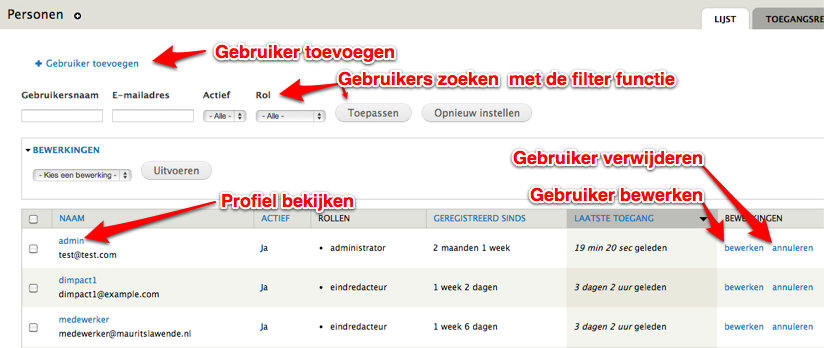
\includegraphics[width=\textwidth]{img/gebruikers1.png}
\end{center}

\subsubsection{Gebruikers toevoegen}

Gebruikers kunnen aangemaakt worden via de frontend(registratie) en via de backend. Deze paragraaf beschrijft hoe je manueel gebruikers kunt toevoegen via de backend. 

Ga naar 'Personen' en klik vervolgens op 'Gebruiker toevoegen', of ga direct naar \drupalpath{admin/people/create}.

Vul alle verplichte velden in en selecteer eventueel welke rol de gebruiker dient te hebben.
Klik onderaan de pagina op 'Nieuw account aanmaken' om de gebruiker toe te voegen.

\subsubsection{Gebruikers bewerken}

Ga naar 'Personen' en klik bij de betreffende gebruiker in de meest rechter kolom op 'bewerken' om het account te gaan bewerken. 
Bewerk het account naar wens en klik vervolgens onderdaan de pagina op de knop 'Opslaan' om de wijzigingen op te slaan.

\subsubsection{Gebruikers verwijderen}

Ongewenste gebruikers accounts kunnen verwijderd worden uit de database; de volgende manier is de meest makkelijke:
Ga naar 'Personen' en kruis in de meest linker kolom aan welke gebruiker je wilt gaan verwijderen, het is mogelijk om meerdere gebruikers tegelijk te verwijderen. Selecteer bij 'Update-instellingen' welke actie je wilt gaan uitvoeren, klik in dit geval op 'Geselecteerde gebruikersaccounts annuleren'. Om de gebruiker(s) daadwerkelijk te verwijderen uit de database klik je op de knop 'Bijwerken'. Let op: deze actie is permanent en kan niet (zomaar) ongedaan worden gemaakt. 



\section{User security}\label{usersecurity}

Het hoofdstuk \emph{User security} omschrijft het beheer ten behoeve van security aangaande sessies van gebruikers.

\subsection{Password policy}\label{passwordpolicy}

De Password policy module maakt het mogelijk om een specifiek niveau van wachtwoordcomplexiteit af te dwingen voor de gebruikerswachtwoorden in het systeem. Een policy bestaat uit instellingen voor rollen, verloop en beperkingen/eisen. Deze module is uitgeschakeld in de standaardconfiguratie, maar kan per gemeente worden ingesteld.

Wanneer de module aan staat kan men naar \emph{Instellingen}, \emph{Personen} en dan op \emph{Password policy} om de instellingen te wijzigen. Een nieuwe policy wordt aangemaakt via het tabblad \emph{Toevoegen}, of ga direct naar \drupalpath{admin/config/people/password_policy/add}.

Bestaande gebruikers kunnen worden verplicht om hun bestaande wachtwoord opnieuw in te stellen. Zie het derde tabblad. (Of ga direct naar \drupalpath{admin/config/people/password_policy/password_change}.)

Algemene configuratie voor verloop, zichtbaarheid en e-mailmeldingen gebeurt op het tabblad \emph{Instellingen}. Deze is rechtstreeks te bereiken via \drupalpath{admin/config/people/password_policy}.

\textbf{Let op! Een standaard verplichting tot wachtwoordwijziging in het CMS en een eventueel gebruikt Lightweight Directory Access Protocol (LDAP) kunnen conflicteren.}

\subsection{Secure pages}\label{securepages}

Voor bepaalde websites zal gebruik worden gemaakt van SSL. Dit kan zo worden ingericht dat:

\begin{itemize}
\item bezoekers automatisch op https terecht komen wanneer ze op de website terecht komen of inloggen;
\item session cookies niet over http verstuurd worden;
\item bezoekers automatisch op https terecht komen wanneer ze ingelogd zijn (op https) en ze bezoeken een pagina over http.
\end{itemize}

In Drupal wordt de settings.php aangepast. In een module wordt code toegevoegd om een ssl cookie te zetten wanneer men op ssl zit. Deze wordt gebruikt om bezoekers op http te redirecten naar https indien ze daar mogelijk ingelogd zijn. Als laatste wordt de Secure pages module ingezet om ervoor te zorgen dat bezoekers automatisch op https terecht komen wanneer ze inloggen of de website bezoeken.

Voor de Drupal-configuratie ga naar \emph{Instellingen}, klik op \emph{Systeem} en dan op \emph{Secure pages}. Of ga rechtstreeks naar \drupalpath{admin/config/system/securepages}.

\section{Site management}\label{sitemanagement}

Het hoofdstuk �Site management� omschrijft alle relevante aspecten van het beheer van de website. Hieronder valt bijvoorbeeld het menu en subsite management .

\section{Menu}\label{menu}
Via een aparte sectie in de beheeromgeving kunnen de beschikbare menu's worden aangepast. Het menu systeem staat in Drupal los van de inhoud (nodes). Om een pagina in het menu toe te voegen zal eerst de pagina toegevoegd moeten worden en kan daarna het menu-item worden aangemaakt.

\subsection{Menu-items toevoegen}\label{menuitemstoevoegen}
menu items toevoegen tekst

\subsection{Menu-items bewerken}\label{menuitemsbewerken}
menu items bewerken tekst
\subsection{Nieuwsbrief}
\pvelist{ \pve{4.25} }

De module ProRail Newsletter maakt gebruik van Drupal webforms voor het aanbieden 
van in- en uitschrijfformulieren voor nieuwsbrieven. Elke nieuwsbrief heeft 
\'{e}\'{e}n aanmeldformulier en \'{e}\'{e}n afmeldformulier. Aanmeldingen zijn 
eenvoudigweg inzendingen van de aanmeldformulieren. Er wordt niet voorzien in een 
koppeling naar een backendsysteem voor verzending, aanmeldingen dienen handmatig 
gedownload te worden als CSV-bestand (zie sectie \ref{sec:inzienaanmeldingen}). 
De module vult de webformulieren op twee belangrijke punten aan:

\begin{itemize}
\item Er wordt per aanmelding een uniek \emph{token} (een tekenreeks van 
willekeurige tekens) aangemaakt, dat meegestuurd moet worden in de 
bevestigingsemail (hiertoe moet de waarde van het tokenveld expliciet in de emailtemplate worden opgenomen) en er wordt in een bevestigingspagina voorzien, waarin 
het token verwerkt wordt en bij een juist token het veld \emph{Bevestigd} bij de aanmelding op 
\emph{Ja} wordt gezet (zie sectie \ref{sec:vereistenaanmeldformulieren}).
Op deze wijze is het niet mogelijk om een email-adres aan te melden via het 
formulier zonder toestemming van degene die werkelijk toegang heeft tot het 
email-adres. 
\item Bij het invullen van een afmeldingsformulier worden aanmeldingen voor het opgegeven 
email-adres (d.w.z. inzendingen van het bijbehorende aanmeldformulier) verwijderd.
\end{itemize}

\subsubsection{Standaard oplevering}
Bij oplevering is er als voorbeeld voorzien in twee aanmeldformulieren en een 
afmeldformulier. Het formulier \emph{Aanmelden nieuwsbrief} is ook daadwerkelijk 
geconfigureerd als aanmeldformulier, het formulier \emph{Aanmelden nieuwsbrief 
eenvoudig} is uitsluitend ter voorbeeld. Het afmeldformulier is gekoppeld aan 
het formulier \emph{Aanmelden nieuwsbrief}.
Afmeldingen kunnen, maar hoeven niet bekeken te worden; ze worden automatisch 
verwerkt, mits voldaan is aan de voorwaarden voor aan- en afmeldformulieren 
zoals hieronder opgesomd.  

\subsubsection{Inzien aanmeldingen}
\label{sec:inzienaanmeldingen}
Als voorbeeld bekijken we hoe de aanmeldingen voor de nieuwsbrief van het 
formulier \emph{Aanmelden nieuwsbrief} ingezien kunnen worden (dit is standaard webform-functionaliteit 
en werkt dus ook voor willekeurige andere webformulieren).

1. Zoek het formulier, bijvoorbeeld via de tab Webformulieren onder Inhoud
\begin{center}
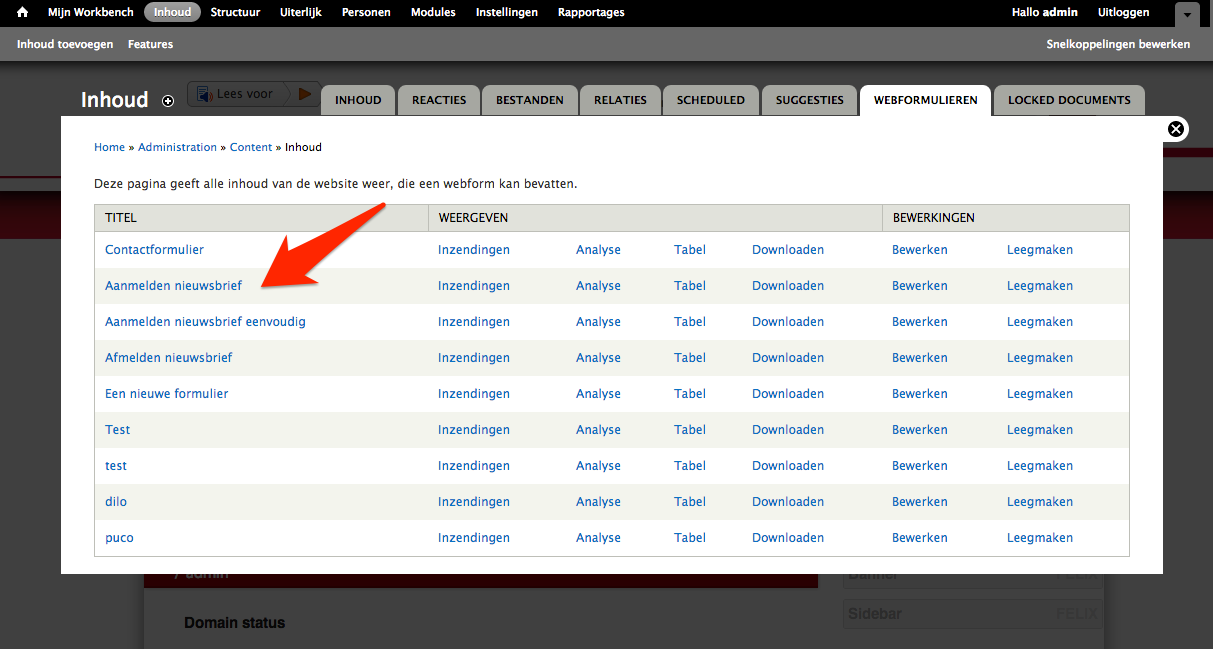
\includegraphics[width=\textwidth]{img/nieuwsbrief/form_aanmelden_nieuwsbrief.png}
\end{center}

2. Klik op de link Tabel
\begin{center}
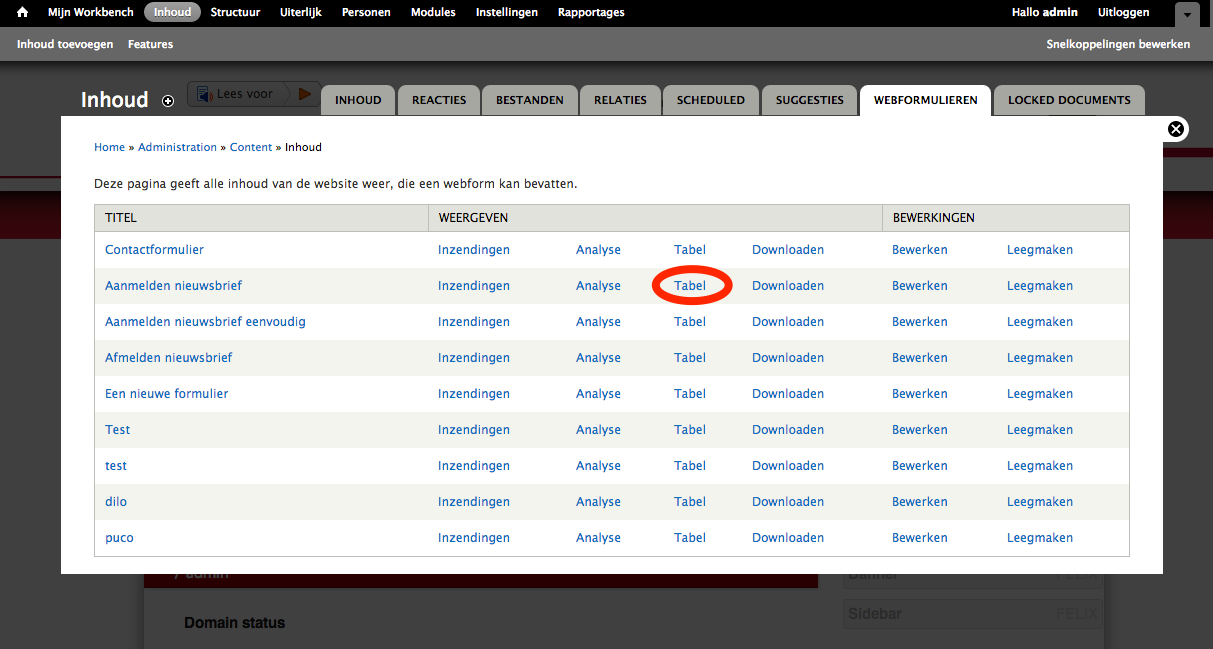
\includegraphics[width=\textwidth]{img/nieuwsbrief/aanmelden_nieuwsbrief_tabellink.png}
\end{center}

3. Een tabel met inzendingen verschijnt.
\begin{center}
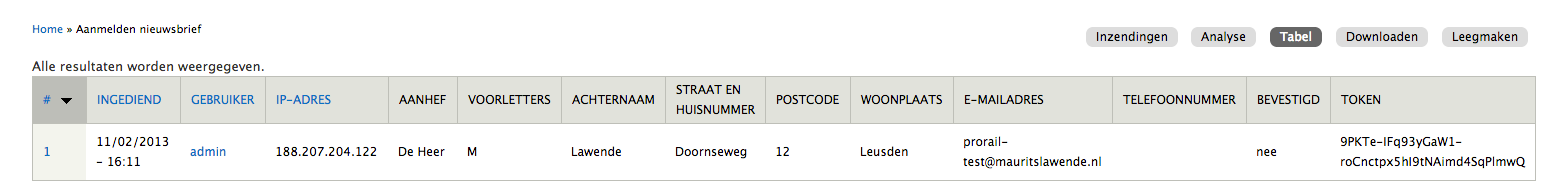
\includegraphics[width=\textwidth]{img/nieuwsbrief/aanmelden_nieuwsbrief_inzendingen.png}
\end{center}

4. De inzendingen kunnen gedownload worden als CSV-bestand op de link Download
\begin{center}
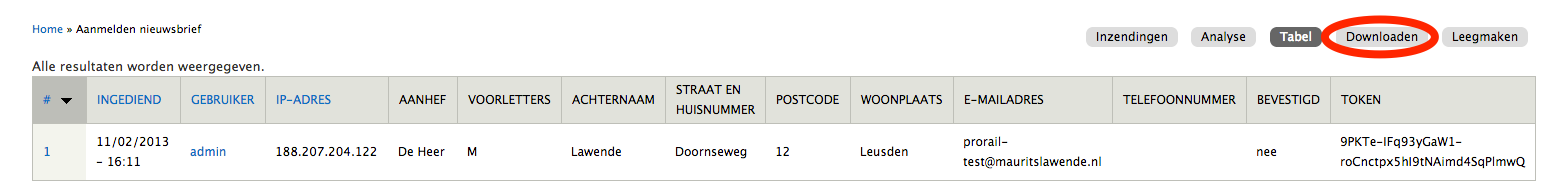
\includegraphics[width=\textwidth]{img/nieuwsbrief/aanmelden_nieuwsbrief_download.png}
\end{center}

Op dit scherm zijn een aantal instellingen mogelijk met bestrekking tot het te 
genereren export-bestand, zoals het scheidingsteken tussen waardes, welke waardes 
ge\"{e}xporteerd moeten worden en welke inzendingen gedownload moeten worden, zoals 
alleen nieuwe inzendingen, alle inzendingen, of een specifiek aantal inzendingen.

\textbf{Let op:} De download bevat alle aanmeldingen, inclusief de 
onbevestigde aanmeldingen. Het is dus bij verdere verwerking van het 
export-bestand van belang dat onbevestigde aanmeldingen worden uitgefilterd 
(dat zijn dus de aanmeldingen waarbij de kolom \emph{Bevestigd} niet op 
\emph{ja} staat).

N.b. Op het download-scherm kan gekozen worden voor het bestandsformaat 
\emph{Microsoft Excel}. Deze optie kan beter niet gebruikt worden, want de enige 
aanpassing die aan het gegenereerde bestand wordt gedaan is het veranderen van de 
bestandsnaamextensie in 
xls. De inhoud van het bestand blijft gelijk, waardoor het geen valide XLS-bestand is.

\subsubsection{Vereisten aanmeldformulieren}
\label{sec:vereistenaanmeldformulieren}
Aanmeldformulieren kunnen als normale webformulieren worden aangemaakt, mits ze aan 
een aantal eisen voldoen (op deze vereisten is geen actieve controle bij het selecteren 
van het formulier in de beheer-interface).

\begin{itemize}
\item Een veld met de machinenaam \emph{email}, dat het aangemelde email-adres bevat. Dit dient een veld van het type \emph{email} te zijn;
\item Een \emph{verborgen} veld met de machinenaam \emph{bevestigd}. Hiervoor moet 
de instelling \emph{veilige waarde} gebruikt worden zodat de 
waarde niet van buitenaf meegestuurd kan worden door middel van een malafide inzending. 
De standaard-waarde van dit veld moet op \emph{nee} ingesteld worden (in feite 
zijn hier geen beperkingen op anders dan dat de standaard-waarde niet \emph{ja}
mag zijn, want dat is de waarde die door de module wordt ingevuld bij bevestiging van 
de inschrijving).
\item Een \emph{verborgen} veld met de machinenaam \emph{token}. Dit veld wordt gebruikt voor het opslaan 
en controleren van het aangemaakte token. 
Ook hiervoor dient de instelling \emph{veilig waarde} gebruikt te worden. De 
standaard-waarde hoeft niet ingesteld te worden.
\item Een bevestigingsemail voor de gebruiker met daarin een bevestigingslink. De 
be\-ves\-ti\-gings\-link heeft de volgende vorm:
\url{http://www.prorail.nl/nieuwsbrief/bevestigen/\%value[token]}
Het voorbeeldformulier \emph{Aanmelden nieuwsbrief} bevat ook een voorbeeld van 
de bevestigingsemail met de token op de juiste manier erin opgenomen.
\end{itemize}

Naast deze velden kunnen eventueel andere velden naar keuze worden toegevoegd. Zo 
heeft het standaard opgeleverde aanmeldformulier velden voor postadres-gegevens. 
Aangeraden wordt om zo min mogelijk informatie van de gebruiker te vragen, zodat 
de drempel om voor een nieuwsbrief aan te melden zo laag mogelijk is.

\begin{figure}[p]
\centering
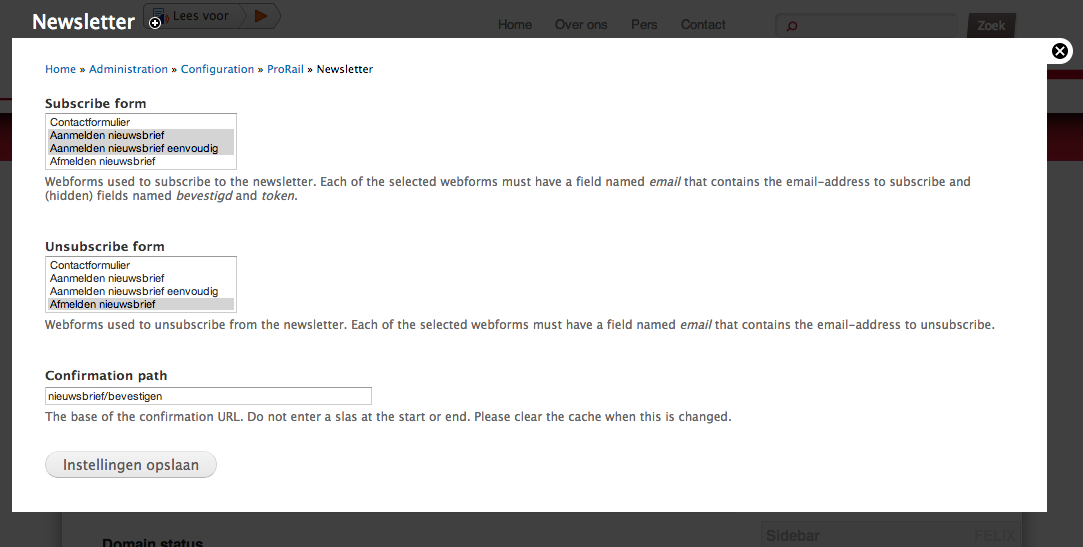
\includegraphics[width=\textwidth]{img/nieuwsbrief/nieuwsbrief_admin.png}
\end{figure}

\subsubsection{Vereisten afmeldformulieren}
\label{sec:vereistenafmeldformulieren}
De enige vereiste voor afmeldformulieren is dat ze een veld hebben met de 
machinenaam \emph{email} van het type \emph{email}. Extra velden kunnen naar 
eigen inzicht worden toegevoegd, bijvoorbeeld velden om een reden voor afmelding 
kenbaar te maken.

\subsubsection{Beheerinterface}
De beheer-interface van de module is te vinden onder Instellingen, ProRail, 
Newsletter.
De volgende instellingen zijn te maken:

\begin{itemize}
\item Het kiezen van webformulieren die dienst doen als aanmeldformulier (let op de vereisten 
zoals vermeld in \ref{sec:vereistenaanmeldformulieren}, of e.e.a. zal niet naar 
behoren werken).
\item Per aanmeldformulier een bijbehorend afmeldformulier (let op de vereisten 
zoals vermeld in \ref{sec:vereistenafmeldformulieren}).
\item Het instellen van het bevestigings-pad, dat wil zeggen de URL die de 
bevestigingen dient te verwerken. Dit is de link die vermeld dient te worden in de 
bevestigingsemail, die verantwoordelijk is voor het verwerken van aanmeldingstokens. 
Normaal gesproken hoeft dit niet aangepast te worden.
\end{itemize}

\subsubsection{Settings}

De module is instelbaar op admin/config/prorail/newsletter. Hier zijn de volgende zaken in te stellen:

\begin{enumerate}
\item Welke formulieren gelden als inschrijfformulier. Deze formulieren dienen een veld voor het email-adres te hebben met als sleutelveld 'email' en een tweetal verborgen velden, met de keys 'bevestigd' en 'token'. 'token' wordt bij indienen gevult met een unieke string, die in de bevestigingsemail wordt opgenomen in een link waarmee de aanmelding bevestigd moet worden (zie verder). 'bevestigd' wordt op 'ja' gezet zodra deze link bezocht is.

\item Welke formulieren gelden als afmeldformulier. Een email-adres ingevuld in het formulier-element met de sleutelveld 'email' heeft tot gevolg dat inzendingen van de aanmeldformulieren met dat email-adres worden verwijderd.

\item De basis voor bevestigings-URLs. Hier wordt het aangemaakte token aan vastgeplakt. Bijvoorbeeld: "nieuwsbrief/bevestigen". Het is van belang dat de URL die in de email wordt gezet hiermee overeenkomt. (Indien dit wordt verandert moet de cache gelegd worden omdat de menu router-tabel opnieuw opgebouwd moet worden).
\end{enumerate}

Voor de bevestigingsemail wordt de normale Webforms email-voorziening gebruikt. De bevestigingstoken is daar beschikbaar als value[token]. Dit is voor de huidige aanmeldformulieren al juist ingesteld.

\subsubsection{Formulieren nieuwsbrieven}

Een ingelogde gebruiker kan het formulier invullen. Er wordt dan geen e-mail verstuurd. Wel zie je de confirmatiepagina die reguliere gebruikers ook zien, waar staat dat er een e-mail is verstuurd (let dus op: dit gebeurt niet als je als content beheerder het formulier hebt ingevuld.).

Als ingelogde gebruiker kun je ook verplichte velden overslaan.

\begin{figure}[p]
\centering
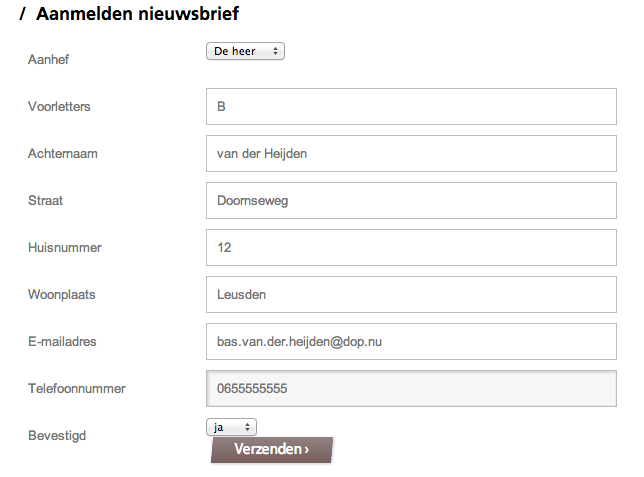
\includegraphics[width=\textwidth]{img/nieuwsbrief/nieuwsbrief_formulier.png}
\end{figure}


\subsection{Dominion}\label{dominion}
De \emph{Dominion} module wordt gebruikt voor het aanmaken van subsites. Ga naar \drupalpath{admin/structure/dominion} voor een overzicht van alle subsites. Het aanmaken van een subsite kan serveraanpassingen vereisen. Dit is zeker het geval wanneer een SSL certificaat op een van de (sub)sites actief is.

\bigskip

\begin{center}
	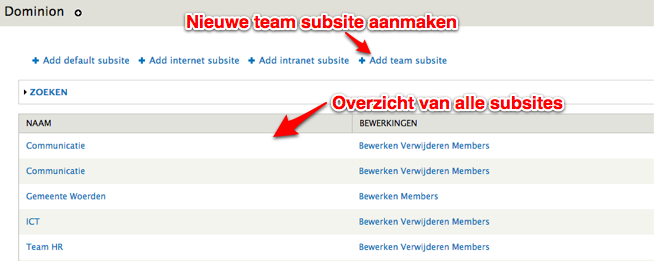
\includegraphics[width=\textwidth]{img/dominion1.png}
\end{center}

\subsubsection{Subsite toevoegen}\label{teamsubsitetoevoegen}
Klik op \emph{Add (internet/intranet/team) subsite} om een nieuwe subsite toe te voegen. 

Onder \emph{Domain type} staan maximaal drie keuzes. Niet alle keuzes kunnen actief zijn.

\begin{itemize}
\item Use a subdomein of .\drupalpath{}. Hiermee kan je subsites aanmaken waarvan de naam \emph{voor} het domein gezet worden. Dat kan dus \emph{intranet}.\drupalpath{} worden.
\item Use a custom domainname. Hier kan je een eigen domein opgeven die helemaal losstaat van het huidige domein. Let wel op dat hiervoor serveraanpassingen vereist zijn.
\item Use a directory. Hiermee kan je subsites aanmaken waarvan de naam \emph{achter} het domein gezet worden. Dat kan dus \drupalpath{}\emph{intranet} worden. Wanneer deze optie geselecteerd wordt zullen er een extra opties getoond worden. Kies bij \emph{Domein} voor het domein waar het achter moet komen. Kies bij \emph{Map} de url, in het voorbeeld zou dat dus \emph{intranet} zijn. 
\end{itemize}

\bigskip

\begin{enumerate}
\item Vul bij het veld \emph{Naam} een naam in voor de subsite.
\item Kies het juiste \emph{Domain type}.
\item Specificeer eventueel de overige opties.
\item Klik op de knop \emph{Opslaan} om de subsite toe te voegen .
\end{enumerate}

\bigskip

\begin{center}
	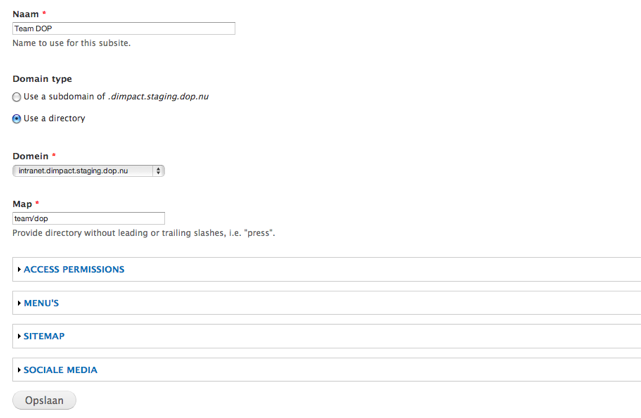
\includegraphics[width=\textwidth]{img/dominion2.png}
\end{center}

\subsubsection{Team members beheren}\label{teammembersbeheren}
Aan elke subsite kunnen \emph{Members} worden toegevoegd.

\bigskip

Klik op \emph{Members} bij de betreffende subsite om \emph{Members} toe te voegen.

\begin{center}
	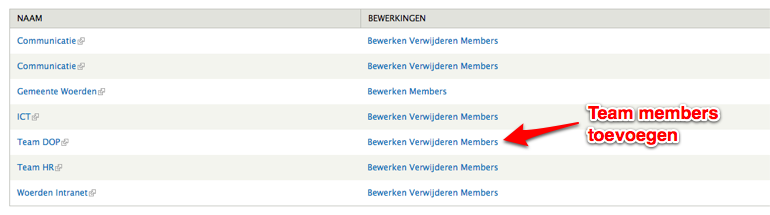
\includegraphics[width=\textwidth]{img/dominion3.png}
\end{center}

\bigskip
Op deze pagina is een lijst te vinden van de huidige teamleden.
Klik op "Add member" om een gebruiker aan de subsite toe te voegen.
Vul de gebruikersnaam of e-mail adres in, selecteer eventueel een domein specifieke rol (bijv. "teamlid") en klik vervolgens op de knop \emph{Toevoegen} om de gebruiker toe te voegen aan de lijst van \emph{Members}.

\bigskip

\begin{center}
	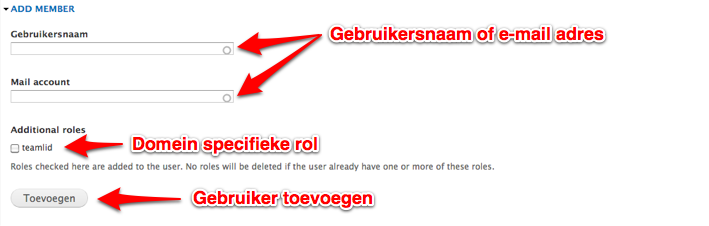
\includegraphics[width=\textwidth]{img/dominion4.png}
\end{center}


\subsection{Flexible blokken}\label{felix}
Het is voor redacteuren mogelijk om blokken de plaatsen op pagina's. Hiermee krijgt de redacteur enige vrijheid over de indeling van de pagina. Hier zijn wel beperkingen van toepassing volgens het grafisch ontwerp.

Door met de muis over de grijze balk te gaan verschijnt er een tandwieltje, als je daarop klikt dan verschijnt er een optie \emph{Blok toevoegen}. Hier kan een keuze gemaakt worden om een enkel item weer te geven op de website, dit zijn \emph{Nodetypes}, of een aantal items, zoals bijvoorbeeld \emph{Het laatste nieuws}.

\begin{center}
	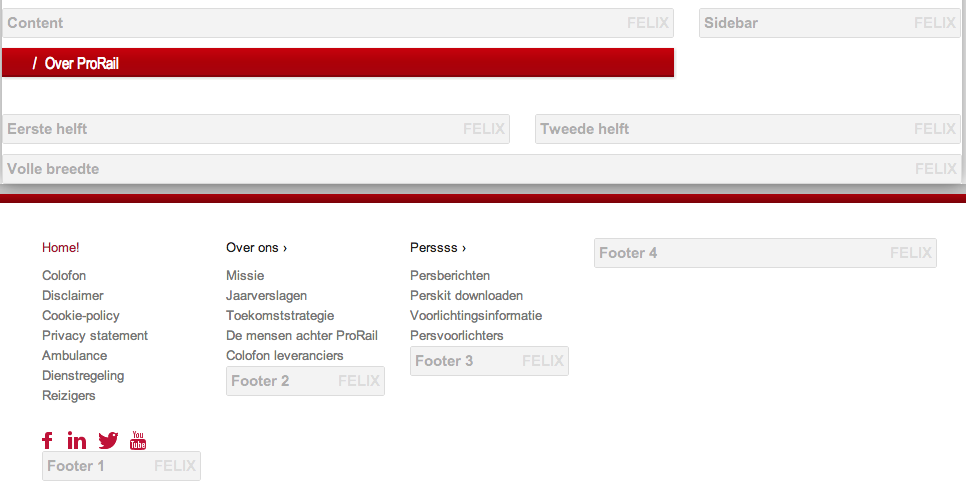
\includegraphics[width=\textwidth]{img/felix.png}
\end{center}
\subsection{Social media}

Ter ondersteuning van het delen op social media wordt voorzien in de volgende zaken:
\begin{itemize}
\item Share buttons
\item Mogelijkheid om widgets in HTML code te plaatsen
\item RSS feeds
\end{itemize}

\subsubsection{Share buttons}

De share buttons geven de mogelijkheid om de pagina te delen op de verschillende sociale media. Hierin kunnen de volgende buttons worden ingesteld:
\begin{itemize}
\item Facebook
\item Google+
\item LinkedIn
\item Twitter
\item Delen op Facebook (widget)
\item Twitteren (widget)
\end{itemize}

Bij oplevering van de standaarddistributie worden de specifieke share links aangezet. De widgets worden niet ingesteld. Deze kunnen bij implementatie van de gemeentesites makkelijk worden aangezet. De theming zal wel geschikt worden gemaakt voor het grotere formaat van deze widgets.

Buttons worden op alle nodetypes toegevoegd die een detailpagina hebben.

Per subsite wordt instelbaar of de share buttons direct zichtbaar zijn of onder een overlay komen. In het laatste geval is een enkele "delen" link beschikbaar waarmee de overlay geopend kan worden. Voor deze instelling wordt een custom \emph{dominion functie} aangemaakt met de systeemnaam \texttt{sharelink}. In het theme kan dan gebruik gemaakt worden van de functie \texttt{dominion\_has\_function} om te bepalen of de overlay gebruikt moet worden.

\subsubsection{Widgets in HTML-code}

Eindredacteuren krijgen de mogelijkheid om zelf HTML widgets te plaatsen in de body tekst\seeone{invoerformaten}.

\subsubsection{Externe RSS-feeds}

Via de \usemodule{views} module i.c.m. de \usemodule{views\_rss} module worden RSS feeds ingesteld. De volgende feeds worden aangemaakt:
\begin{enumerate}
\item Laatste nieuwsberichten
\item Actuele evenementen
\item Laatste bekendmakingen
\item Laatst gewijzigde pagina's
\end{enumerate}
De views worden gesorteerd op publicatiedatum (1 t/m 3) of datum laatst gewijzigd (4). De RSS feed laat altijd 20 items zien.

Nieuwe RSS feeds kunnen niet door de gemeente aangemaakt worden.


\subsection{Google Analytics}\label{googleanalytics}
De bezoekersstatistieken van de \drupalpath website en haar subsites worden bijgehouden d.m.v. Google Analytics. Het \emph{Intranet} wordt bijgehouden door \emph{Piwik}.

De module \emph{Googleanalytics}  wordt gebruikt voor het koppelen van je Google Analytics account. Ga naar \drupalpath{admin/config/system/googleanalytics} om uw Google Analytics account te kopellen aan Dimpact. 

Vul bij het veld \emph{Web Property ID} je eigen Google ID code in. 

Klik vervolgens onderaan de pagina op de knop \emph{Instellingen opslaan} om de instellingen op te slaan.
\subsection{Sitemap}\label{sitemap}
De sitemap wordt standaard ingesteld tijdens de installatie van Dimpact. Mocht je de sitemap toch naar wens willen aanpassen dan kun je dit doen via de volgende link: \drupalpath{admin/config/search/sitemap}

In dit formulier kun je aangeven wat er in de sitemap moet komen te staan. Voer bij \emph{Paginatitel} een titel voor de pagina in. Onder \emph{Sitemap bericht} kan je een tekst plaatsen die op de pagina zichtbaar is. 

Onder \emph{SITEMAP INHOUD} kan je kiezen voor de volgende instellingen. \emph{Geef de voorpagina weer}, plaats een link naar de voorpagina. \emph{Menu's die in de sitemap moeten worden opgenomen}, geef aan welke menu's getoond moeten worden als lijstweergave op de sitemap. \emph{Geef FAQ inhoud weer}, toont een lijst met FAQ items. \emph{Categorieen die in de sitemap moeten worden opgenomen}, toont een lijst met taxonomietermen die binnen de vocabulaires vallen.

Onder \emph{CATEGORIE-INSTELLINGEN} stel je de weergavemodus in voor de te tonen taxonomietermen. \emph{Show node counts by categories} toont het aantal gekoppelde nodes aan een taxonomieterm. \emph{Categories depth} geef de diepte op tot op welk niveau termen opgehaald moeten worden. \emph{thresholds} geven aan vanaf hoeveel gekoppelde items de term weergegeven moet worden.

Onder \emph{RSS-INSTELLINGEN} stel je de instellingen in voor de RSS feed. Onder \emph{CSS SETTINGS} kan je opgeven of je het CSS bestand bij de RSS feed wilt inladen.

Klik onderaan de pagina op de knop \emph{Instellingen opslaan} om te instellingen op te slaan. De sitemap wordt dan beschikbaar op /sitemap.
\subsection{Cache}\label{cache}
\emph{Drupal} maakt gebruik van \emph{caching} functionaliteit. Het doel van \emph{caching} is de website sneller maken. De cache slaat bijvoorbeeld pagina's op in de database. Op deze manier kan de website, gebruikmakend van de cache, de al eerder opgeslagen pagina een stuk sneller tonen. 

Na het wijzigen van bijvoorbeeld content of menu-items moet de cache handmatig verschoont worden, indien je de wijzigingen \emph{direct} zichtbaar wilt maken. 

\textbf{Cache opschonen:}

\begin{enumerate}
\item Ga naar  \drupalpath{admin/config/development/performance}
\item Klik op de knop \emph{Alle caches legen}
\item Wacht op de succes melding, dit duurt ongeveer een halve minuut
\end{enumerate}

\begin{center}
	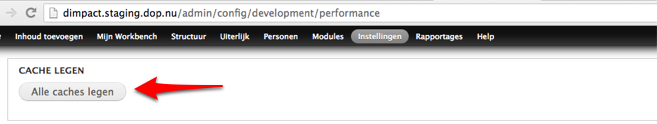
\includegraphics[width=\textwidth]{img/cache.png}
\end{center}

\section{Site algemeen}\label{sitealgemeen}
In dit hoofdstuk worden de overige functionaliteiten van de website uitgelegd.


\subsection{Voorpagina}\label{voorpagina}

\subsubsection{Grid}

De template van de website bestaat uit een grid, een soort geraamte. Het grid is opgebouwd uit verschillende regio's. In elke regio kunnen blokken geplaatst worden. In de paragraaf \emph{Felix}\seeone{felix} staat beschreven hoe en welke je blokken kunt toevoegen aan een regio. 

\bigskip

\begin{center}
	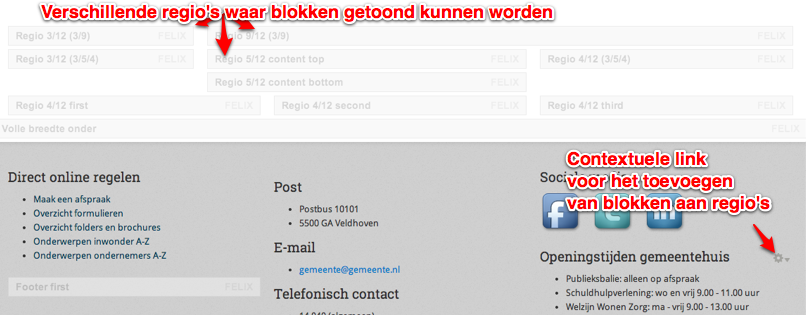
\includegraphics[width=\textwidth]{img/grid1.png}
\end{center}

\subsubsection{Blokken}

In het onderstaande afbeelding worden alle bestaande blokken op voorpagina in het kort toegelicht.

\bigskip

\begin{center}
	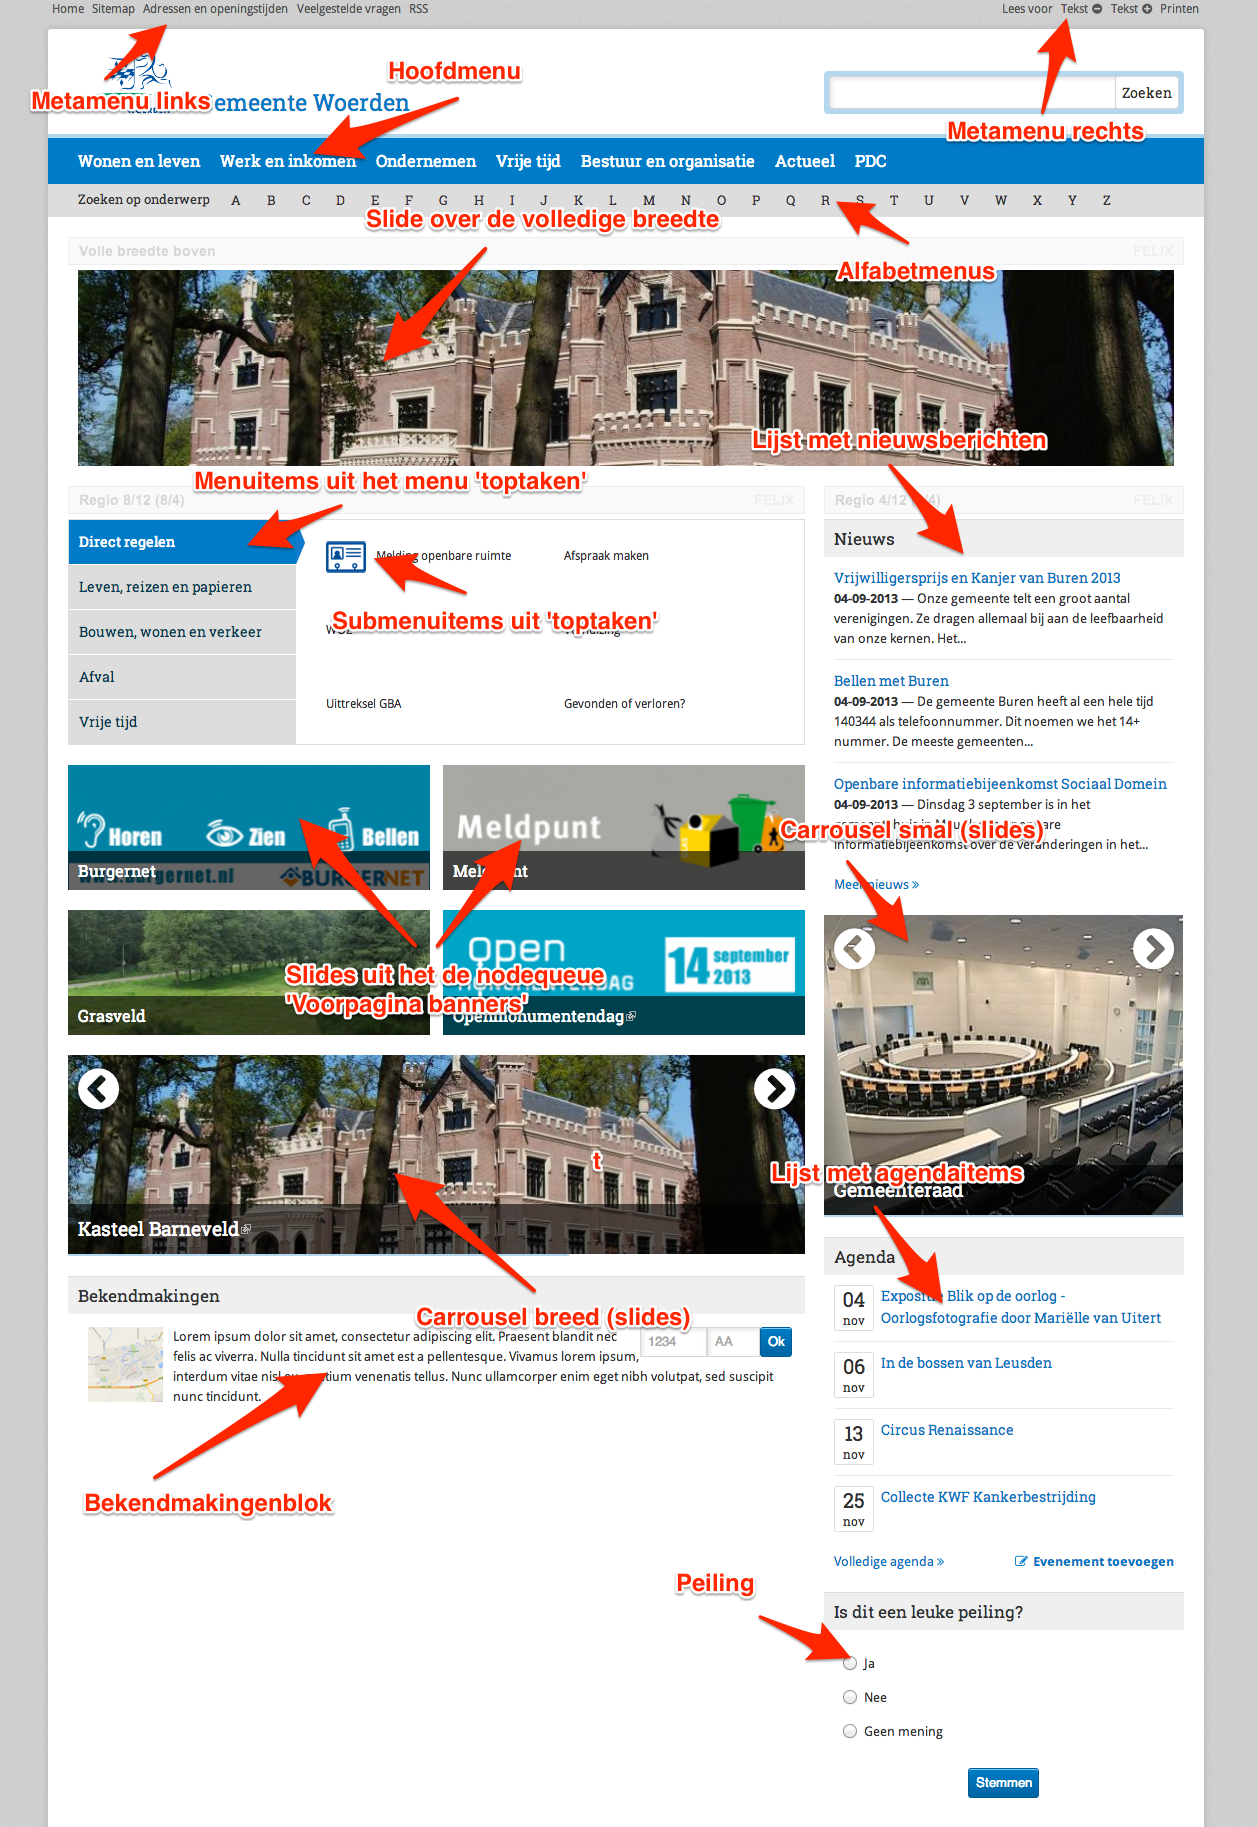
\includegraphics[width=\textwidth]{img/voorpagina.png}
\end{center}

\subsubsection{Footer}

In het onderstaande afbeelding worden alle bestaande blokken in de footer in het kort toegelicht. De footer bestaat uit 3 regio's waar blokken in gezet kunnen worden. De standaard configuratie is links een menu blok "Direct online regelen", in het hoofdstuk \emph{Menu}\seeone{menu} wordt beschreven hoe het menu te bewerken is. In de middenkolom staat blok met redactionele content. In de rechterkolom staan twee blokken; het eerste blok is het Dominion social blok. In paragraaf \emph{Social media}\seeone{socialmedia} staat beschreven hoe deze opties te beheren zijn. Daaronder staat nog een blok met redactionele content. Naast de standaard geconfigureerde blokken zijn in de drie regio's ook nog Felix blokken te zetten. 

\bigskip

\begin{center}
	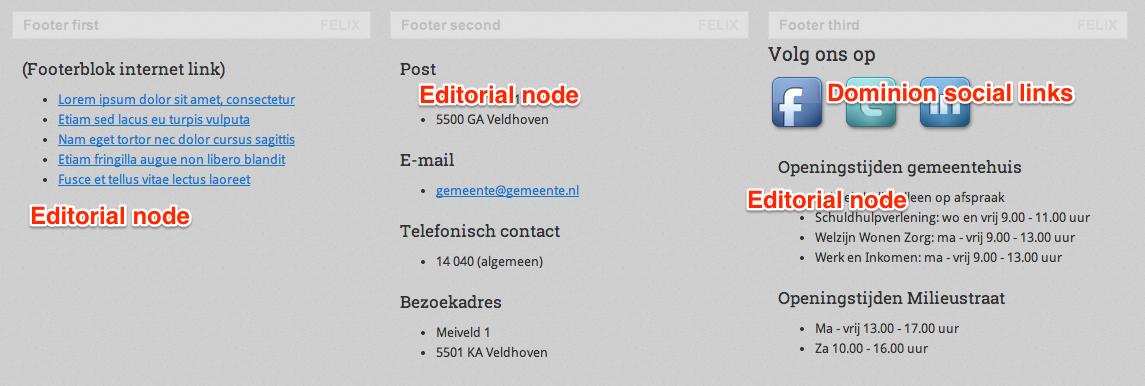
\includegraphics[width=\textwidth]{img/voorpagina3.png}
\end{center}

\subsection{Taxonomie}\label{taxonomie}

Taxonomie wordt gebruikt voor lijsten van woorden. Bijvoorbeeld: de lijst �FAQ categorie�n� bevat de woorden 'Netwerk' en 'Werkplekken'. Taxonomie lijsten kunnen altijd aangepast worden.

\bigskip

\begin{center}
	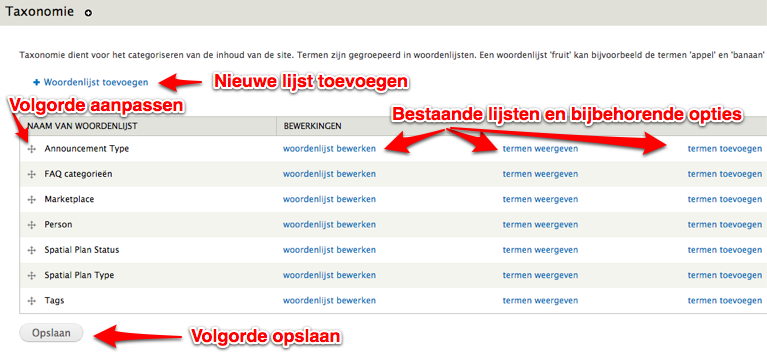
\includegraphics[width=\textwidth]{img/taxonomie2.png}
\end{center}

\subsubsection{Woorden aan woordenlijsten toevoegen}

Ga naar het overzicht van alle woordenlijsten. Klik op 'Termen toevoegen' bij de lijst waaraan je woorden wil toevoegen. Vul bij het veld 'Naam' het woord in en vul eventueel een beschrijving in. Klik onderaan de pagina op de knop 'Opslaan' om het woord aan de lijst toe te voegen. Herhaal deze stappen om meerdere woorden toe te voegen aan de woordenlijst. 

\subsubsection{Woorden in woordenlijsten bewerken}

Het is mogelijk om specifieke woorden uit lijsten te bewerken. Klik op 'Termen weergeven' bij de betreffende lijst.
Klik op 'Bewerken' bij het betreffende woord, vervolgens kun je de wijzigingen doorvoeren. Klik op de knop 'Opslaan' om de wijzigingen op te slaan.

\subsubsection{Woorden uit woordenlijsten verwijderen}

Het is mogelijk om specifieke woorden uit lijsten te verwijderen. Klik op 'Termen weergeven' bij de betreffende lijst.
Klik op 'Bewerken' bij het betreffende woord, om het woord te verwijderen klik je onderaan de op de knop 'Verwijderen'. Na het bevestigen zal het woord definitief en onherstelbaar verwijderd worden.


\subsection{Zoeken}\label{zoeken}

Voor \drupalpath wordt de \emph{Solr module} gebruikt, deze module vervangt de standaard \emph{Drupal Search module}. 
De \emph{Solr module} biedt naast de standaard zoek functionaliteit ook meer geavanceerde functionaliteiten zoals zoeken in bijlagen, markeren van zoekwoorden en de mogelijkheid tot het aanpassen van de \emph{Bias settings}. 

\subsubsection{Bias settings}

\emph{Bias settings} maken het mogelijk inhoud voorrang te geven in de zoekresultaten. Je kunt bijvoorbeeld het inhoudstype \emph{Nieuws} meer punten geven dan het inhoudstype \emph{Bekendmaking}. Hoe hoger het aantal toegekende punten hoe meer voorrang het krijgt. 

Ga naar \drupalpath{admin/config/search/apachesolr} en klik vervolgens op \emph{Bias} bij de betreffende website om de \emph{Bias settings} aan te passen. Let op: het is niet aangeraden om zonder voldoende kennis deze settings aan te passen.

\begin{center}
	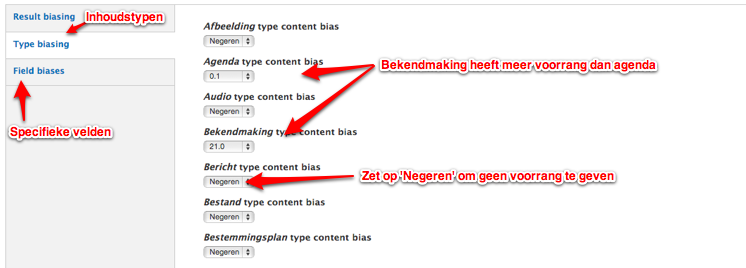
\includegraphics[width=\textwidth]{img/bias.png}
\end{center}

Klik na het bewerken op de knop \emph{Instellingen opslaan} om de \emph{Bias settings} op te slaan. 

\subsubsection{Content uitsluiten van zoekmachine}

Het is mogelijk om specifieke nodes uit te sluiten van indexatie in de interne zoekmachine. Klik onderaan het bewerkformulier op het tabblad \emph{Uitsluiten uit zoekresultaten} en vink de checkbox aan, zie onderataand afbeelding.

\begin{center}
	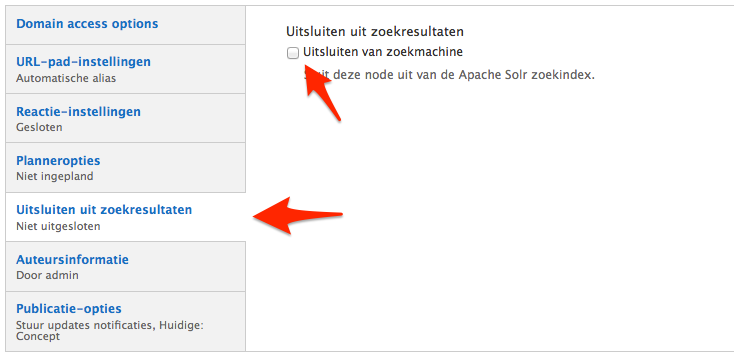
\includegraphics[width=\textwidth]{img/solr-exclude.png}
\end{center}

\subsubsection{Synoniemen beheren}

Solr biedt ondersteuning voor synoniemen. Hiermee kan worden ingesteld dat een zoekopdracht naar "i-pad" ook inhoud met de tekst "ipad" wordt opgenomen in de resultaten.

De synoniemen zijn te beheren via Drupal. Ga hiervoor naar \\ \drupalpath{admin/config/search/apachesolr/synonyms}. Op deze pagina is een lijst te vinden met de huidige synoniemen. Deze kunnen hier worden aangepast of uit de lijst worden gehaald. Onder de lijst is een formulier zichtbaar waarmee nieuwe synoniemen toegevoegd kunnen worden. Het trefwoord is het originele woord (bijv. "ipad") en de synoniemen worden ingevoerd als een komma gescheiden lijst (bijv. "i-pad, i pad").

Nieuwe synoniemen treden niet direct in werking. De lijst wordt iedere nacht doorgezet naar de Solr server. In dit proces wordt tevens de ingestelde lijst samengevoegd met de basislijst (generieke lijst voor alle gemeentes).

\subsection{Afbeeldingsstijlen}\label{afbeeldingsstijlen}

Afbeeldingsstijlen worden gebruikt voor het weergeven van afbeeldingen. Verschillende afbeeldingsstijlen maken het mogelijk een afbeelding op een andere manier (ander formaat bijvoorbeeld) te tonen dan het origineel. 

\subsubsection{Banner}

Banner 

\subsubsection{Full width}

Full width 

\subsubsection{List thumbnail}

List thumbnail 

\subsubsection{Node thumbnail}

Node thumbnail 

\subsubsection{Origineel}

Origineel 

\subsubsection{Overige onderwerp}

Overige onderwerp 

\subsubsection{Portret}

Portret 

\subsubsection{Slide 9/3}

Slide 9/3 

\subsubsection{galleryformatterslide}

galleryformatter slide 

\subsubsection{galleryformatterthumb}

galleryformatter thumb 

\subsubsection{Thumbnail}

thumbnail 

\subsubsection{Medium}

medium 

\subsubsection{Large}

large 

\subsubsection{linkitthumb}

linkut thumb 

\subsubsection{squarethumbnail}

square thumbnail 

\section{Imports}

Dimpact bevat import modules om een deel van de inhoud te importeren uit gemeentelijke en landelijke voorzieningen. Het gaat hier om automatische processen die in de \emph{cron} worden gestart. De \emph{cron} is een proces dat periodiek op de achtergrond draait. Aangezien het om automatische imports gaat zijn de beheeropties minimaal. Wel is het mogelijk om imports handmatig te starten.

\subsection{GVOP}

De GVOP koppeling importeert regelingen (CVDR) en bekendmakingen. Hiervan wordt de dienst gebruikt op \texttt{zoek.officielebekendmakingen.nl}.

Bekendmakingen komen in het nodetype \emph{Bekendmaking} en regelingen (CVDR) in het nodetype \emph{Regeling}.

Een handmatige import kan gestart worden op de volgende pagina: \\
\drupalpath{admin/config/content/gvop}

\subsection{Atos eSuite}

De importmodule van de Atos eSuite importeert producten en vraag antwoord combinaties (VAC's) die aanwezig zijn in de eSuite. Producten worden ge\"{i}mporteerd als \emph{Product} node en VAC's als \emph{VAC}.

De export van de Atos eSuite bevat geen categorie\"{e}n. Na de import kunnen deze handmatig toegevoegd worden door de \emph{Product} nodes te bewerken. De categorie wordt niet overschreven door de import. Andere velden die wel uit de import mogen niet in Drupal worden aangepast, aangezien deze wijzigingen wel overschreven zullen worden.

Een handmatige import kan gestart worden op de volgende pagina: \\
\drupalpath{admin/config/content/atos-esuite}

\subsection{DURP}

Deze module importeert bestemmingsplannen via de standaard \emph{Digitale Uitwisseling in Ruimtelijke Processen}, oftewel \emph{DURP}. De gemeentes bieden zelf de plannen aan op een publiekelijk beschikbare URL. De XML bestanden zelf volgen de \emph{IMRO2012} standaard. Een voorbeeld van een dergelijk bestand is hier te vinden:
\texttt{http://ro.zwolle.nl/manifest/manifest2012.xml}.

Ge\"{i}mporteerde items zijn in Drupal terug te vinden als \emph{Bestemmingsplan} nodes.

Een handmatige import kan gestart worden op de volgende pagina: \\
\drupalpath{admin/config/content/durp}

\section{Rechten en rollen}

Drupal heeft de mogelijkheid om meerdere rollen aan te maken. Aan elke rol kunnen vervolgens rechten worden toegekend. Welke rechten er zijn is afhankelijk van de gebruikte modules een aanwezige contenttypes. Een gebruiker kan aan meerdere rollen worden gekoppeld. Doorgaans wordt \'{e}\'{e}n rol gebruikt voor redacteuren / beheerders.

\subsection{Rollen}

De volgende rollen zijn gedefin\"{i}eerd:
\begin{itemize}
\item Beheerder \\
	Heeft toegang tot beheerpagina's en kan alle inhoud, subsites en gebruikers beheren.
\item Eindredacteur \\
	Kan alle inhoud en team subsites beheren.
\item Redacteur \\
	Kan inhoud beheren op eigen domeinen. Kan wel inhoud aanmaken, maar niet publiceren.
\item Medewerker \\
	Toegang tot bepaalde functionaliteit die exclusief is voor medewerkers (bijv. wiki).
\item Teamlid \\
	Kan inhoud beheren binnen eigen team subsites.
\end{itemize}

\subsection{Inhoudstypen}

Hier worden de rechten op inhoud beschreven. Het aanmaken en publiceren zijn losse rechten. Wel kunnen aanmaken en niet kunnen publiceren betekend dat wijzigingen door een andere rol goedgekeurd moeten worden\seeone{workflow}. Bij het bewerken en verwijderen is er onderscheid tussen het muteren van eigen inhoud of het muteren van alle inhoud. Bij elke permissie zijn de rollen afgekort tot de eerste letter.
\begin{itemize}
\item \textbf{B}eheerder
\item \textbf{E}indredacteur
\item \textbf{R}edacteur
\item \textbf{M}edewerker
\item \textbf{T}eamlid
\end{itemize}
\begin{tabularx}{\textwidth}{ | p{5cm} |X|X|X|X|X|X| }
  \hline
  \textbf{Inhoudstype} & \rotatebox[origin=l]{90}{\textbf{Aanmaken}} & \rotatebox[origin=l]{90}{\textbf{Bewerken}} & \rotatebox[origin=l]{90}{\textbf{Alles bewerken}} & \rotatebox[origin=l]{90}{\textbf{Verwijderen}} & \rotatebox[origin=l]{90}{\textbf{Alles verwijderen }} & \rotatebox[origin=l]{90}{\textbf{Publiceren}} \\ \hline
  Agenda & BERT & BERT & BE & BERT & BE & BE \\ \hline
  Bekendmaking & B & B & B & B & B & B \\ \hline
  Intranet bericht & BET & BET & BE & BET & BE & BE \\ \hline
  Bestand & BET & BET & BE & BET & BE & BE \\ \hline
  Bestemmingsplan & BE & BE & BE & BE & BE & BE \\ \hline
  Blog & BERT & BERT & BE & BERT & BE & BE \\ \hline
  Editorial & BER & BER & BE & BER & BE & BE \\ \hline
  Eenvoudige pagina & BER & BER & BE & BER & BE & BE \\ \hline
  FAQ & BER & BER & BE & BER & BE & BE \\ \hline
  Forumonderwerp & BE & BE & BE & BE & BE & BE \\ \hline
  Foto & BE & BE & BE & BE & BE & BE \\ \hline
  Forumonderwerp & BE & BE & BE & BE & BE & BE \\ \hline
  Marktplaats & BERM & BERM & BE & BERM & BE & BE \\ \hline
  Nieuws & BER & BER & BE & BER & BE & BE \\ \hline
  Onderwerp & BE & BE & BE & BE & BE & BE \\ \hline
  Peiling & BER & BER & BE & BER & BE & BE \\ \hline
  Persoon & BER & BER & BE & BER & BE & BE \\ \hline
  Product & BER & BER & BE & BER & BE & BE \\ \hline
  Regeilng & B & B & B & B & B & B \\ \hline
  RSS & BE & BE & BE & BE & BE & BE \\ \hline
  RSS Source & BE & BE & BE & BE & BE & BE \\ \hline
  Slide & BER & BER & BE & BER & BE & BE \\ \hline
  VAC & BE & BE & BE & BE & BE & BE \\ \hline
  Webformulier & BE & BE & BE & BE & BE & BE \\ \hline
  Wiki & BERMT & BERMT & BE & BERMT & BE & BE \\ \hline
\end{tabularx}

\clearpage
\subsection{Permissies}

Het volgende overzicht geeft aan welke rollen toegang hebben tot bepaald acties.
Bij elke permissie zijn de rollen afgekort tot de eerste letter.

\begin{tabularx}{\textwidth}{ | p{10cm} | X | } \hline 
\textbf{Actie} & \textbf{Rollen} \\ \hline
Beheerinterface gebruiken 	& BER \\ \hline
Content uitsluiten van zoekmachine 	& BE \\ \hline
Andere invoerformaten kiezen 	& BERT \\ \hline
Reageren op content 	& BERTM \\ \hline
Eigen reacties bewerken 	& B \\ \hline
Blokken en context beheren 	& BE \\ \hline
Contextual links gebruiken 	& BER \\ \hline
Team subsites beheren 	& BE \\ \hline
Subsite menu's beheren 	& BER \\ \hline
Cron settings aanpassen 	& B \\ \hline
Felix blokken beheren op eigen domein 	& BER \\ \hline
Felix blokken beheren op alle domeinen 	& BE \\ \hline
Toegang tot alle uploads 	& B \\ \hline
Bestanden uploaden 	& BERT \\ \hline
Eigen bestanden aanpassen 	& BERT \\ \hline
Alle bestanden aanpassen 	& BE \\ \hline
Volledige HTML gebruiken 	& BE \\ \hline
Gefilterde HTML gebruiken 	& BERTM \\ \hline
Forums beheren 	& B \\ \hline
Vertalingen aanpassen 	& BE \\ \hline
MailChimp campagnes beheren 	& B \\ \hline
Inloggen als andere gebruikers 	& B \\ \hline
Externe video's toevoegen (via media) 	& BER \\ \hline
Nodequeues aanpassen 	& BER \\ \hline
URL Aliasen beheren 	& BE \\ \hline
Stemmen van de poll bekijken 	& BER \\ \hline
Publiceren onder embargo 	& BER \\ \hline
Termen in woordenlijsten beheren 	& BE \\ \hline
Gebruikers beheren 	& B \\ \hline
Gebruikersprofielen bekijken 	& BE \\ \hline
Inzendingen van formulieren bekijken 	& BE \\ \hline
Workbench gebruiken 	& BER \\ \hline
\end{tabularx}



\clearpage

\end{document}
